%!TEX root=../../main.tex
\begin{chapterpage}{Inference for categorical data}
  \chaptertitle{Inference for\\[4mm]categorical data}
  \label{inferenceForCategoricalData}
  \chaptersection{singleProportion}
  \chaptersection{differenceOfTwoProportions}
  \chaptersection{twoWayTablesAndChiSquare}
  \chaptersection{oneWayChiSquare}
  \chaptersection{caseControlStudies}
  \chaptersection{inferenceBinaryData}
  \chaptersection{infForPropNotes}
  \chaptersection{infForPropExercises}
\end{chapterpage}
\renewcommand{\chapterfolder}{ch_inference_for_props_oi_biostat}

\chapterintro{{\large Previous chapters discussed methods of inference for numerical data; in this chapter, those methods are extended to categorical data, such as binomial proportions or data in two-way tables. While various details of the methods may change, such as the calculations for a test statistic or the distributions used to find a $p$-value, the core ideas and principles behind inference remain the same.

Categorical data arise frequently in medical research because disease outcomes and patient characteristics are often recorded in natural categories such as types of treatment received, whether or not disease advanced to a later stage, or whether or not a patient responded initially to a treatment. In the simplest settings, a binary outcome (yes/no, success/failure, etc)  is recorded for a single group of participants, in hopes of learning more about the population from which the participants were drawn.  The binomial distribution is often used for the statistical model in this setting, and inference about the binomial probability of success provides information about a population proportion $p$.   In more complex settings, participant characteristics are recorded in a categorical variable with two or more levels, and the outcome or response variable itself has two or more levels.  In these instances, data are usually summarized in two-way tables with two or more rows and two or more columns.

As with all methods of inference, it is important to understand how the data were collected and whether the data may be viewed as a random sample from a well-identified population, at least approximately.  This issue is at least as important as the formulas for test statistics and confidence intervals, and is often overlooked.

Be careful about the notation in this chapter---since $p$ is the standard notation for a population proportion and for a probability, $p$ does double duty in this chapter as a population parameter and significance level.}}


%__________________
\section{Inference for a single proportion}
\label{singleProportion}

Advanced melanoma is an aggressive form of skin cancer that until recently was almost uniformly fatal.  In rare instances, a patient's melanoma stopped progressing or disappeared altogether when the patient's immune system successfully mounted a response to the cancer. Those observations led to research into therapies that might trigger an immune response in cancer.  Some of the most notable successes have been in melanoma, particularly with two new therapies, nivolumab and ipilimumab\footnote{The -mab suffix in these therapies stands for monoclonal antibody, a therapeutic agent made by identical immune cells that are all clones of a unique parent cell from a patient.}.

A 2013 report in the New England Journal of Medicine by Wolchok et al. reported the results of a study in which patients were treated with both nivolumab and ipilimumab.\footnote{N Engl J Med 2013;369:122-33. DOI: 10.1056/NEJMoa1302369}   Fifty-three patients were given the new regimens concurrently, and the response to therapy could be evaluated in 52 of the 53.  Of the 52 evaluable patients, 21 (40\%) experienced a response according to commonly accepted criteria.  In previous studies, the proportion of patients responding to one of these agents was 30\% or less.  How might one compare the new data to past results?

The data from this study are binomial data, with success defined as a response to therapy. Suppose the number of patients who respond in a study like this is represented by the random variable $X$, where $X$ is binomial with parameters $n$ (the number of trials, where each trial is represented by a patient) and $p$ (the unknown population proportion of response). From formulas discussed in Chapter~\ref{modeling}, the mean of $X$ is $np$ and the standard deviation of $X$ is $\sqrt{np(1-p)}$.

Inference about $p$ is based on the sample proportion $\hat{p}$, where $\hat{p} = X/n$. In this case, $\hat{p} = 21/52 = 0.404$. If the sample proportion is nearly normally distributed, the normal approximation to the binomial distribution can be used to conduct inference; this method is commonly used.  When $X$ does not have an approximately normal distribution, exact inference can  based on the binomial distribution for $X$.  Both the normal approximation and exact methods are covered in this chapter.

\subsection{Inference using the normal approximation}
\label{normalApproxSingleBinomial}

A \term{sample proportion} can be described as a sample mean. If each success in the melanoma data  is represented as a \texttt{1} and each failure as a \texttt{0}, then the sample proportion is the mean of the 52 numerical outcomes:
\begin{eqnarray*}
\hat{p} = \frac{\ 0 + 1 + 1 + \cdots + 0\ }{52} = 0.404.
\end{eqnarray*}
The distribution of $\hat{p}$ is nearly normal when the distribution of successes and failures is not too strongly skewed.

\textD{\newpage}

\index{sampling distribution!sample proportion}

\begin{onebox}{Conditions for the sampling distribution of $\pmb{\hat{\MakeLowercase{p}}}$ being nearly normal}
The sampling distribution for $\hat{p}$, calculated from a sample of size $n$ from a population with a success proportion $p$, is nearly normal when
\begin{enumerate}
\item the sample observations are independent and
\item at least 10 successes and 10 failures are expected in the sample, i.e. $np\geq10$ and $n(1-p)\geq10$. This is called the \term{success-failure condition}.
\end{enumerate}
If these conditions are met, then the sampling distribution of $\hat{p}$ is approximately normal with mean $p$ and standard error
\index{standard error (SE)!single proportion}
\begin{eqnarray}
SE_{\hat{p}} = \sqrt{\frac{p(1-p)}{n}}.
\label{seOfPHat}
\end{eqnarray}
\end{onebox}%
\marginpar[\raggedright\vspace{-53mm}

$\hat{p}$\vspace{0mm}\\\footnotesize sample\\proportion\vspace{3mm}\\\normalsize$p$\vspace{0mm}\\\footnotesize population\\proportion]{\raggedright\vspace{-53mm}

$\hat{p}$\vspace{0mm}\\\footnotesize sample\\proportion\vspace{3mm}\\\normalsize$p$\vspace{0mm}\\\footnotesize population\\proportion}

When conducting inference, the population proportion $p$ is unknown. Thus, to construct a confidence interval, the sample proportion $\hat{p}$ can be substituted for $p$ to check the success-failure condition and compute the standard error. In a hypothesis test, $p_0$ is substituted for $p$.

\subsubsection{Confidence intervals for a proportion}
\label{confIntForPropSection}

\index{point estimate!single proportion}
\index{confidence interval!single proportion}

When using the normal approximation to the sampling distribution of $\hat{p}$, a confidence interval for a proportion has the same structure as a confidence interval for a mean; it is centered at the point estimate, with a margin of error calculated from the standard error and appropriate $z^{\star}$ value.  The formula for a 95\% confidence interval is
\[
  \hat{p} \pm 1.96 \sqrt{\frac{\hat{p}(1-\hat{p})}{n}}.
\]

\begin{examplewrap}
\begin{nexample}{Using the normal approximation, construct an approximate 95\% confidence interval for the response probability for patients with advanced melanoma who were administered the combination of nivolumab and ipilimumab.}

The independence and success-failure assumptions should be checked first.  Since the outcome of one patient is unlikely to influence that of other patients, the observations are independent.  The success-failure condition is satisfied since $n\hat{p} = (52)(.404) = 21  > 10$ and $n\hat{p}(1 - \hat{p}) = (52)(.596) = 31  > 10$.

The point estimate for the response probability, based on a sample of size $n = 52$, is $\hat{p} = 0.404$. For a 95\% confidence interval, $z^{\star} = 1.96$. The standard error is estimated as: $\sqrt{\frac{\ \hat{p}(1-\hat{p})\ }{n}} = \sqrt{\frac{(0.404)(1-0.404)}{52}} = 0.068$.  The confidence interval is
\[0.404 \pm 1.96 (0.068) \rightarrow (0.27, 0.54) \]
The approximate 95\% confidence interval for $p$, the population response probability of melanoma patients to the combination of these new drugs, is (0.27, 0.54) or (27\%, 54\%).  
\end{nexample}
\end{examplewrap}

\textD{\newpage}

\begin{exercisewrap}
\begin{nexercise}
In New York City on October 23rd, 2014, a doctor who had recently been treating Ebola patients in Guinea went to the hospital with a slight fever and was subsequently diagnosed with Ebola. Soon after, a survey conducted by the Marist Poll, an organization with a carefully designed methodology for drawing random samples from identified populations, found that 82\% of New Yorkers favored a "mandatory 21-day quarantine for anyone who has come in contact with an Ebola patient."\footnotemark{} a) Verify that the sampling distribution of $\hat{p}$ is nearly normal. b) Construct a 95\% confidence interval for $p$, the proportion of New York adults who supported a quarantine for anyone who has come into contact with an Ebola patient.\footnotemark{}
\end{nexercise}
\end{exercisewrap}
\addtocounter{footnote}{-1}%
\footnotetext{\oiRedirect{textbook-maristpoll_ebola_201410}{Poll ID NY141026 on maristpoll.marist.edu}.}%
\addtocounter{footnote}{1}%
\footnotetext{a) The poll is based on a simple random sample and consists of fewer than 10\% of the adult population of New York, which makes independence a reasonable assumption. The success-failure condition is satisfied since, $1042(0.82) > 5$ and $1042(1-0.82) > 5$. b) $0.82 \pm 1.96\sqrt{\frac{0.82(1-0.82)}{1042}} \rightarrow (0.796, 0.844)$.}

Did the participants in the melanoma trial constitute a random sample?  Patients who participate in clinical trials are unlikely to be a random sample of patients with the disease under study since the patients or their physicians must be aware of the trial, and patients must be well enough to travel to a major medical center and be willing to receive an experimental therapy that may have serious side effects.  

Investigators in the melanoma trial were aware that the observed proportion of patients responding in a clinical trial may be different than the hypothetical response probability in the population of patients with advanced melanoma. Study teams try to minimize these systematic differences by following strict specifications for deciding whether patients are eligible for a study. However, there is no guarantee that the results observed in a sample will be replicated in the general population.

Small, initial studies in which there is no control group, like the one described here, are early steps in exploring the value of a new therapy and are used to justify further study of a treatment when the results are substantially different than expected.  The largest observed response rate in previous trials of 30\% was close to the lower bound of the confidence interval from the study (27\%, 54\%), so the results were considered adequate justification for continued research on this treatment.

\subsubsection{Hypothesis testing for a proportion}
\label{htForPropSection}
\index{hypothesis testing!single proportion}

Just as with inference for population means, confidence intervals for population proportions can be used when deciding whether to reject a null hypothesis. It is useful in most settings, however, to calculate the $p$-value for a test as a measure of the strength of the evidence contradicting the null hypothesis.

When using the normal approximation for the distribution of $\hat{p}$ to conduct a hypothesis test, one should always verify that $\hat{p}$ is nearly normal under $H_0$ by checking the independence and success-failure conditions. Since a hypothesis test is based on the distribution of the test statistic under the null hypothesis, the success-failure condition is checked using the null proportion $p_0$, not the estimate $\hat{p}$. 

According to the normal approximation to the binomial distribution, the number of successes in $n$ trials is normally distributed with mean $np_0$ and standard deviation $\sqrt{np(1-p_0)}$. This approximation is valid when $np_0$ and $n(1-p_0)$ are both at least 10.\footnote{The normal approximation to the binomial distribution was discussed in Section~\ref{binomialModel} of Chapter~\ref{modeling}.} 

\textD{\newpage}

Under the null hypothesis, the sample proportion $\hat{p} = X/n$ is approximately distributed as 
\[N \left(p_0, \sqrt{\frac{p_0(1-p_0)}{n}} \right).\]
The test statistic $z$ for the null hypothesis $H_0: p = p_0$ based on a sample of size $n$ is 
\begin{align*}
  z &= \dfrac{\text{point estimate - null value}}{SE} \\
    &= \dfrac{\hat{p} - p_0}{\sqrt{\frac{(p_0)(1-p_0)}{n}}}. 
\end{align*}

\begin{examplewrap}
\begin{nexample}{Suppose that out of a cohort of 120 patients with stage 1 lung cancer at the Dana-Farber Cancer Institute (DFCI) treated with a new surgical approach, 80 of the patients survive at least 5 years, and suppose that National Cancer Institute statistics indicate that the 5-year survival probability for stage 1 lung cancer patients nationally is 0.60. Do the data collected from 120 patients support the claim that the DFCI population treated with this new form of surgery has a different 5-year survival probability than the national population? Let $\alpha = 0.10$, since this is an early study of the new surgery.}

Test the hypothesis $H_0: p = 0.60$ versus the alternative, $H_A:  p \neq 0.60$, using $\alpha = 0.10$. If we assume that the outcome of one patient at DFCI does not influence the outcome of other patients, the independence condition is met, and the success-failure condition is satisfied since $(120)(0.60) = 80 > 5$ and $(120)(1-0.60) = 40 > 5.$ The test statistic is the $z$-score of the point estimate: 
\[z = \dfrac{\text{point estimate - null value}}{SE} = \dfrac{0.67 - 0.60}{\sqrt{\frac{(0.60)(1-0.60)}{120}}} = 1.57. \]
The $p$-value is the probability that a standard normal variable is larger than 1.57 or smaller than -1.57, $P(|Z| > 1.57) = 0.12$ ; since the $p$-value is greater than 0.10, there is insufficient evidence to reject $H_0$ in favor of $H_A$. There is not convincing evidence that the survival probability at DFCI differs from the national survival probability.  Had a more traditional 0.05 significance level been used, the data would be even less convincing. 
\end{nexample}
\end{examplewrap}

\begin{examplewrap}
\begin{nexample}{Using the data from the study in advanced melanoma, use the normal approximation to the sampling distribution of $\hat{p}$ to test the null hypothesis that the response probability to the novel combined therapy is 30\% against a one-sided alternative that the response proportion is greater than 30\%. Let $\alpha = 0.10$.}

The test statistic has value 
\[
z = (0.404 - 0.30)/\sqrt{(0.30)(0.70)/52} = 1.64. 
\] 
The one-sided $p$-value is $P(Z \geq 1.64) = 0.05$; there is sufficient evidence to reject the null hypothesis at $\alpha = 0.10$. This is an example of where a two-sided test and a one-sided test yield different conclusions.
\end{nexample}
\end{examplewrap}

\index{data!nhanes}

\textD{\newpage}

\begin{exercisewrap}
\begin{nexercise}
One of the questions on the National Health and Nutrition Examination Survey (introduced in Chapter~\ref{inferenceForNumericalData}) asked participants whether they participated in moderate or vigorous intensity sports, fitness, or recreational activities. In a random sample of 135 adults, 76 answered "Yes" to the question. Based on this evidence, are a majority of American adults physically active?\footnotemark{}
\end{nexercise}
\end{exercisewrap}
\footnotetext{The observations are independent. Check success-failure: $np_0 = n(1-p_0) = 135(0.5) > 10$. $H_0: p = 0.5$; $H_A: p > 0.5$. Calculate the $z$-score: $z = \frac{0.56 - 0.50}{\sqrt{\frac{0.5(1-0.5)}{135}}} = 1.39$. The $p$-value is 0.08. Since the $p$-value is larger than 0.05, there is insufficient evidence to reject $H_0$; there is not convincing evidence that a majority of Americans are physically active, although the data suggest that may be the case.}


\subsection{Inference using exact methods}
\label{exactMethodsSingleBinomial}

When the normal approximation to the distribution of $\hat{p}$ may not be accurate, inference is based on exact binomial probabilities. Calculating confidence intervals and $p$-values based on the binomial distribution can be done by hand, with tables of the binomial distribution, or (more easily and accurately) with statistical software. The logic behind computing a $p$-value is discussed here, but the formulas for a confidence interval are complicated and are not shown.

The $p$-value for a hypothesis test corresponds to the sum of the probabilities of all events that are as or more extreme than the sample result. Let $X$ be a binomial random variable with parameters $n$ and $p_0$, where $\hat{p} = x/n$ and $x$ is the observed number of events. If $\hat{p} \leq p_0$, then the one-tail probability equals $P(X \leq x)$; if $\hat{p} > p_0$, then the one-tail probability equals $P(X \geq x)$. These probabilities are calculated using the approaches from Chapter~\ref{modeling}. Two-tailed probabilities are calculated by doubling the appropriate one-tailed value.

\index{data!glioblastoma}

\begin{examplewrap}
\begin{nexample}{In 2009, the FDA Oncology Drug Advisory Committee (ODAC) recommended that the drug Avastin be approved for use in glioblastoma, a form of brain cancer. Tumor shrinkage after taking a drug is called a response; out of 85 patients, 24 exhibited a response. Historically, response probabilities for brain cancer drugs were approximately 0.05, or about 5\%. Assess whether there is evidence that the response probability for Avastin is different from previous drugs. } \label{avastinFDAApproval}	

$H_0: p = 0.05$; $H_A: p \neq 0.05$. Let $\alpha = 0.05$. 

The independence condition is satisfied, but the success-failure condition is not, since $np_0 = (85)(0.05) = 4.25 < 5$, so this is a setting where exact binomial probabilities should be used to calculate a $p$-value.

The sample proportion $\hat{p}$ equals $x/n = 24/85 = 0.28$. Since $\hat{p} > p_0$, calculate the two-sided $p$-value from $2 \times P(X \geq 24)$, where $X \sim \text{Binom}(85, 0.05)$.

Calculating the $p$-value is best done in software; the \textsf{R} command \texttt{pbinom} returns a value of $5.3486 \times 10^{-12}$.\footnotemark{}

The $p$-value is highly significant and suggests that the response probability for Avastin is higher than for previous brain cancer drugs. The FDA staff considered this evidence sufficiently strong to justify approval for the use of the drug, even though the FDA normally requires evidence from two independently conducted randomized trials. 
\end{nexample}
\end{examplewrap}
\footnotetext{\texttt{2*pbinom(q = 23, size = 85, p = 0.05, lower.tail = FALSE)}}

\textD{\newpage}

\begin{exercisewrap}
\begin{nexercise}
Medical consultants assist patients with all aspects of an organ donation surgery, with the goal of reducing the possibility of complications during the medical procedure and recovery. To attract customers, one consultant noted that while the usual proportion of complications in liver donation surgeries in the United States is about 10\%, only 3 out of her 62 clients experienced complications with liver donor surgeries. Is there evidence to suggest that the proportion of complications in her patients is lower than the national average?\footnotemark{}
\end{nexercise}
\end{exercisewrap}
\footnotetext{Assume that the 62 patients in her dataset may be viewed as a random sample from patients receiving a donated liver. The sample proportion $\hat{p} = 3/62 = 0.048$. Under the null hypothesis, the expected number of complications is $62(0.10) = 6.2$, so the normal approximation may not be accurate and it is best to use exact binomial probabilities. Since $\hat{p} \leq p_0$, find the $p$-value by calculating $P(X \leq 3)$ when $X$ has a binomial distribution with parameters $n = 62,\, p = 0.10$: $P(X \leq 3) = 0.121$. There is not sufficient evidence to suggest that the proportion of complications among her patients is lower than the national average.}


\subsection{Choosing a sample size when estimating a proportion}

\index{margin of error|(}
\index{sample size!estimating a proportion|(}

Whenever possible, a sample size for a study should be estimated before data collection begins.  Section \ref{PowerForDifferenceOfTwoMeans} explored the calculation of sample sizes that allow a hypothesis test comparing two groups to have adequate power.  When estimating a proportion, preliminary sample size calculations are often done to estimate a sample size large enough to make the \term{margin of error} $m$ in a confidence interval sufficiently small for the interval to be useful. Recall that the margin of error $m$ is the term that is added to and subtracted from the point estimate.  Statistically, this means estimating a sample size $n$ so that the sample proportion is within some margin of error $m$ of the actual proportion with a certain level of confidence. When the normal approximation is used for a binomial proportion, a sample size sufficiently large to have a margin of error of $m$ will satisfy 
\begin{align*}
 m = (z^{\star})(\text{s.e.}(\hat{p})) = z^{\star} \sqrt{\frac{(p)(1 - p)}{n}}. 
\end{align*}
Algebra can be used to show that the above equation implies
\begin{align*}
n = \frac{(z^{\star})^2(p)(1 - p)}{m^2}.
\end{align*}
In some settings a preliminary estimate for $p$ can be used to calculate $n$.  When no estimate is available, calculus can be used to show that $p(1 - p)$ has its largest value when $p = 0.50$, and that conservative value for $p$ is often used to ensure that $n$ is sufficiently large regardless of the value of the unknown population proportion $p$.  In  that case, $n$ satisfies
\begin{align*}
  n \geq \frac{(z^{\star})^2(0.50)(1-0.50)}{m^2} = \frac{(z^{\star})^2}{4m^2}.
\end{align*}

\textD{\newpage}

\begin{examplewrap}
\begin{nexample}{Donor organs for organ transplant are scarce. Studies are conducted to explore whether the population of eligible organs can be expanded. Suppose a research team is studying the possibility of transplanting lungs from hepatitis C positive individuals; recipients can be treated with one of the new drugs that cures hepatitis C. Preliminary studies in organ transplant are often designed to estimate the probability of a successful organ graft 6 months after the transplant.  How large should a study be so that the 95\% confidence interval for the probability of a successful graft at 6 months is no wider than 20\%?}

A confidence interval no wider than 20\% has a margin of error of 10\%, or 0.10.  Using the conservative value p = 0.50,
\[n = \frac{(1.96)^2}{(4)(0.10^2)} =  96.04.\]
Sample sizes are always rounded up, so the study should have 97 patients.  

Since the study will likely yield a value $\hat{p}$ different from 0.50, the final margin of error will be smaller than $\pm 0.10$.
\end{nexample}
\end{examplewrap}

When the confidence coefficient is 95\%, 1.96 can replaced by 2 and the sample size formula reduces to 
\begin{align*}
  n = 1/m^2.
\end{align*}
This remarkably simple formula is often used by practitioners for a quick estimate of sample size.

\index{sample size!estimating a proportion|)}

\index{data!Congress approval rating|(}

\begin{exercisewrap}
\begin{nexercise}
A 2015 estimate of Congress' approval rating was 19\%.\footnotemark{} Using this estimate, how large should an additional survey be to produce a margin of error of 0.04 with 95\% confidence?\footnotemark{}
\end{nexercise}
\end{exercisewrap}
\addtocounter{footnote}{-1}%
\footnotetext{\oiRedirect{textbook-congress_at_19_in_May2015}{www.gallup.com/poll/183128/five-months-gop-congress-approval-remains-low.aspx}}%
\addtocounter{footnote}{1}%
\footnotetext{Apply the formula \\
\begin{align*}
1.96\times \sqrt{\frac{p(1-p)}{n}} \approx
1.96\times \sqrt{\frac{0.19(1-0.19)}{n}} &\leq 0.04 \qquad\to\qquad n \geq 369.5.
\end{align*}
A sample size of 370 or more would be reasonable.}

\index{data!Congress approval rating|)}
\index{margin of error|)}



%__________________
\section{Inference for the difference of two proportions}
\label{differenceOfTwoProportions}

Just as inference can be done for the difference of two population means, conclusions can also be drawn about the difference of two population proportions: $p_1 - p_2$. 

\subsection{Sampling distribution of the difference of two proportions}
\label{samplingDistributionDiffTwoProps}

\index{sampling distribution!difference of two proportions}
\index{point estimate!difference of two proportions}

The normal model can be applied to $\hat{p}_1 - \hat{p}_2$ if the sampling distribution for each sample proportion is nearly normal and if the samples are independent random samples from the relevant populations. 

\begin{onebox}{Conditions for the sampling distribution of $\hat{p}_1 - \hat{p}_2$ to be approximately normal}
The difference $\hat{p}_1 - \hat{p}_2$ tends to follow a normal model when
\begin{itemize}
\setlength{\itemsep}{0mm}
\item each of the two samples are random samples from a population,
\item the two samples are independent of each other, and
\item each sample proportion follows (approximately) a normal model. This condition is satisfied when $n_1p_1, n_1(1 - p_1), n_2 p_2$ and $n_2(1 - p_2)$ are all $\geq 10$.
\end{itemize}
The standard error of the difference in sample proportions is
\index{standard error (SE)!difference in proportions}
\begin{eqnarray}
SE_{\hat{p}_1 - \hat{p}_2}
	= \sqrt{SE_{\hat{p}_1}^2 + SE_{\hat{p}_2}^2}
	= \sqrt{\frac{p_1(1-p_1)}{n_1} + \frac{p_2(1-p_2)}{n_2}},
\label{seForDiffOfProp}
\end{eqnarray}
where $p_1$ and $p_2$ are the population proportions, and $n_1$ and $n_2$ are the two sample sizes.
\end{onebox}


\textD{\newpage}


\subsection{Confidence intervals for $\pmb{\MakeLowercase{p_1 - p_2}}$}
\label{confidenceIntervalsDifferenceProportions}
\index{confidence interval!difference of two proportions}

When calculating confidence intervals for a difference of two proportions using the normal approximation to the binomial, the two sample proportions are used to verify the success-failure condition and to compute the standard error.

\begin{examplewrap}
\begin{nexample}{The way a question is phrased can influence a person's response. For example, Pew Research Center conducted a survey with the following question:\footnotemark{}
\begin{quote}
As you may know, by 2014 nearly all Americans will be required to have health insurance. [People who do not buy insurance will pay a penalty] while [People who cannot afford it will receive financial help from the government]. Do you approve or disapprove of this policy?
\end{quote}
\index{data!health care|(}For each randomly sampled respondent, the statements in brackets were randomized: either they were kept in the order given above, or the order of the two statements was reversed. Figure~\ref{pewPollResultsForRandomizedStatementOrdering} shows the results of this experiment. Calculate and interpret a 90\% confidence interval of the difference in the probability of approval of the policy.}
First the conditions for the use of a normal model must be verified. The Pew Research Center uses sampling methods that produce random samples of the US population (at least approximately) and because each group was a simple random sample from less than 10\% of the population, the observations are independent, both within the samples and between the samples. The success-failure condition also holds for each sample, so the normal model can be used for confidence intervals for the difference in approval proportions.  The point estimate of the difference in support, where $\hat{p}_1$ corresponds to the original ordering and $\hat{p}_2$ to the reversed ordering:
$$\hat{p}_{1} - \hat{p}_{2} = 0.47 - 0.34 = 0.13.$$
The standard error can be computed from Equation~\eqref{seForDiffOfProp} using the sample proportions:
$$SE \approx \sqrt{\frac{0.47(1-0.47)}{771} + \frac{0.34(1-0.34)}{732}} = 0.025.$$
For a 90\% confidence interval, $z^{\star} = 1.65$:
$$\text{point estimate} \ \pm\ z^{\star} \times SE \quad \to \quad 0.13 \ \pm\ 1.65 \times  0.025 \quad \to \quad (0.09, 0.17).$$
With 90\% confidence, the proportion approving the 2010 health care law ranged between 9\% and 17\% depending on the phrasing of the question. The Pew Research Center interpreted this modestly large difference as an indication that for most of the public, opinions were still fluid on the health insurance mandate.  The law eventually passed as the Affordable Health Care Act (ACA).
\index{data!health care|)}
\end{nexample}
\end{examplewrap}
\footnotetext{\oiRedirect{textbook-health_care_bill_2012}{www.people-press.org/2012/03/26/public-remains-split-on-health-care-bill-opposed-to-mandate}. Sample sizes for each polling group are approximate.}

\begin{figure}[h]
\centering
\begin{tabular}{c c c c c}
	& Sample size ($n_i$) & Approve (\%)	& Disapprove (\%)	& Other \\
\hline
Original ordering & 771	& 47	& 49	& 3 \\
Reversed ordering & 732	& 34	& 63	& 3 \\
\hline
\end{tabular}
\caption{Results for a Pew Research Center poll where the ordering of two statements in a question regarding healthcare were randomized.\vspaceB{-2mm}}
\label{pewPollResultsForRandomizedStatementOrdering}
\end{figure}


\textD{\newpage}


\subsection{Hypothesis testing for $\pmb{\MakeLowercase{p_1 - p_2}}$}

%\index{hypothesis test!difference of two proportions}

Hypothesis tests for $p_1 - p_2$ are usually testing the null hypothesis of no difference between $p_1$ and $p_2$; i.e. $H_0:\,p_1 - p_2 = 0$. Under the null hypothesis, $\hat{p}_1 - \hat{p}_2$ is normally distributed with mean 0 and standard deviation $\sqrt{p(1-p)(\frac{1}{n_1} + \frac{1}{n_2})}$, where under the null hypothesis $p = p_1 = p_2$.

Since $p$ is unknown, an estimate is used to compute the standard error of $\hat{p}_1 - \hat{p}_2$; $p$ can be estimated by $\hat{p}$, the weighted average of the sample proportions $\hat{p}_1$ and $\hat{p}_2$:
\[\hat{p} = \dfrac{n_{1}\hat{p}_1 + n_{2}\hat{p}_2}{n_{1} + n_{2}} = \dfrac{x_{1} + x_{2}}{n_{1} + n_{2}}, \]
where $x_1$ is the number of observed events in the first sample and $x_2$ is the number of observed events in the second sample. This pooled proportion $\hat{p}$ is also used to check the success-failure condition.

The test statistic $z$ for testing $H_0:\, p_1 = p_2$ versus $H_A: p_1 \neq p_2$ equals:

\[z = \dfrac{\hat{p}_1 - \hat{p}_2}{\sqrt{\hat{p}(1-\hat{p})\left(\frac{1}{n_1} + \frac{1}{n_2} \right)}}. \]
 
\index{data!mammography|(}
\index{data!breast cancer|(}

\begin{examplewrap}
\begin{nexample}{The use of screening mammograms for breast cancer has been controversial for decades because the overall benefit on breast cancer mortality is uncertain.  Several large randomized studies have been conducted in an attempt to estimate the effect of mammogram screening. A 30-year study to investigate the effectiveness of mammograms versus a standard non-mammogram breast cancer exam was conducted in Canada with 89,835 female participants.\footnotemark{} During a 5-year screening period, each woman was randomized to either receive annual mammograms or standard physical exams for breast cancer.  During the 25 years following the screening period, each woman was screened for breast cancer according to the standard of care at her health care center. \vspace{3mm}

At the end of the 25 year follow-up period, 1,005 women died from breast cancer. The results by intervention are summarized in Figure~\ref{mammogramStudySummaryTable}. \vspace{3mm}

Assess whether the normal model can be used to analyze the study results.}\label{mammogramSuccessFailure}%

Since the participants were randomly assigned to each group, the groups can be treated as independent, and it is reasonable to assume independence of patients within each group.  Participants in randomized studies are rarely random samples from a population, but the investigators in the Canadian trial recruited  participants using a general publicity campaign, by sending personal invitation letters to women identified from general population lists, and through contacting family doctors.  In this study, the participants can reasonably be thought of as a random sample.

The pooled proportion $\hat{p}$ is  

\[\hat{p} = \dfrac{x_{1} + x_{2}}{n_{1} + n_{2}} = \dfrac{500 + 505}{500 + 44,425 + 505 + 44,405} = 0.0112. \]

Checking the success-failure condition for each group: 
\begin{align*}
\hat{p} \times n_{mgm} &= 0.0112 \times \text{44,925} = 503
& (1 - \hat{p}) \times n_{mgm} &= 0.9888 \times \text{44,925} = \text{44,422} \\
\hat{p} \times n_{ctrl} &= 0.0112 \times \text{44,910} = 503
& (1 - \hat{p}) \times n_{ctrl} &= 0.9888 \times \text{44,910} = \text{44,407}
\end{align*}
All values are at least 10. 

The normal model can be used to analyze the study results.
\end{nexample}
\end{examplewrap}
\footnotetext{\oiRedirect{textbook-90k_mammogram_study_2014}{Miller AB. 2014. \emph{Twenty five year follow-up for breast cancer incidence and mortality of the Canadian National Breast Screening Study: randomised screening trial}. BMJ 2014;348:g366 doi: 10.1136/bmj.g366}}

\begin{figure}[h]
	\centering
	\begin{tabular}{rrcc}
		& \multicolumn{3}{c}{Death from breast cancer?} \\
		\cline{2-4}
		& \ \hspace{3mm}\ & Yes & No \\
		\hline
		Mammogram && 500 & 44,425 \\
		Control && 505 & 44,405 \\
		\hline
	\end{tabular}
	\caption{Summary results for the mammogram study.}
	\label{mammogramStudySummaryTable}
\end{figure}

\textD{\newpage}

\begin{examplewrap}
\begin{nexample}{Do the results from the study provide convincing evidence of a difference in the proportion of breast cancer deaths between women who had annual mammograms during the screening period versus women who received annual screening with physical exams?}\label{mammogramExProp}%
The null hypothesis is that the probability of a breast cancer death is the same for the women in the two groups. If group 1 represents the mammogram group and group 2 the control group, $H_0: p_1 = p_2$ and $H_A: p_1 \neq p_2$.  Let $\alpha = 0.05$.

Calculate the test statistic $z$:
\[z = \dfrac{0.01113 - 0.01125}{\sqrt{(0.0112)(1-0.0112)\left(\frac{1}{44,925} + \frac{1}{44,910} \right)}} = -0.17.
\]	
The two-sided $p$-value is $P|Z| \ge 0.17 = 0.8650$,  which is greater than 0.05. There is insufficient evidence to reject the null hypothesis; the observed difference in breast cancer death rates is reasonably explained by chance. 	

Evaluating medical treatments typically requires accounting for additional evidence that cannot be evaluated from a statistical test. For example, if mammograms are much more expensive than a standard screening and do not offer clear benefits, there is reason to recommend standard screenings over mammograms. This study also found that a higher proportion of diagnosed breast cancer cases in the mammogram screening arm (3250 in the mammogram group vs 3133 in the physical exam group), despite the nearly equal number of breast cancer deaths.  The investigators inferred that mammograms may cause over-diagnosis of breast cancer, a phenomenon in which a breast cancer diagnosed with mammogram and subsequent biopsy may never become symptomatic. The possibility of over-diagnosis is one of the reasons mammogram screening remains controversial.
\end{nexample}
\end{examplewrap}

\begin{examplewrap}
\begin{nexample}{Calculate a 95\% confidence interval for the difference in proportions of deaths from breast cancer from the Canadian study.}\label{mammogramExConfInt}%

The independence and random sampling conditions have already been discussed.  The success failure condition should be checked for each sample, since this is not a hypothesis testing context (i.e., there is no null hypothesis). For the mammogram group, $\hat{p}_1 = 0.01113$; $n_1 \hat{p}_1 = (0.1113)(44,925) = 500$ and $n_1 (1 - \hat{p}_1) = 39,925.$ It is easy to show that the success failure condition is holds for the control group as well.

The point estimate for the difference in the probability of death is
$$\hat{p}_{1} - \hat{p}_{2} = 0.01113 - 0.01125 = -0.00012,$$ or 0.012\%.

The standard error for the estimated difference uses the individual estimates of the probability of a death:
$$SE \approx \sqrt{\frac{0.01113(1-0.01113)}{44,925} + \frac{0.01125(1-0.01125)}{44,910}} = 0.0007. $$

The 95\% confidence interval is given by 
$$ -0.00012 \pm (1.96) (0.0007) = (-0.0015, 0.0013).$$

With 95\% confidence, the difference in the probability of death is between -0.15\% and 0.13\%. As expected from the large $p$-value, the confidence interval contains the null value 0.
\end{nexample}
\end{examplewrap}

\index{data!breast cancer|)}
\index{data!mammography|)}


%__________________
\section{Inference for two or more groups}
\label{twoWayTablesAndChiSquare}

The comparison of the proportion of breast cancer deaths between the two groups can also be approached using a two-way contingency table, which contains counts for combinations of outcomes for two variables. The results for the mammogram study in this format are shown in Figure~\ref{mammogramStudySummaryTableWithTotals}.

Previously, the main question of interest was stated as, "Is there evidence of a difference in the proportion of breast cancer deaths between the two screening groups?" If the probability of a death from breast cancer does not depend the method of screening, then screening method and outcome are independent. Thus, the question can be re-phrased: "Is there evidence that screening method is associated with outcome?"

Hypothesis testing in a two-way table assesses whether the two variables of interest are associated (i.e., not independent). The approach can be applied to settings with two or more groups and for responses that have two or more categories. The observed number of counts in each table cell are compared to the number of \term{expected counts}, where the expected counts are calculated under the assumption that the null hypothesis of no association is true. A $\chi^2$ test of significance is based on the differences between observed and expected values in the cells.

\begin{figure}[h]
	\centering
	\begin{tabular}{l| l l l l |l}
		\hline
		Death from BC & \hspace{1mm}  & Yes & No & \hspace{1mm} & Total \\
		\hline
		Mammogram				   &    & 500 & 44,425 & 				&44,925 \\
		Control				   &     & 505	& 44,405    &				& 44,910 \\
		\hline
		Total						   &    & 1,005 & 88,830 & 				& 89,835 \\
		\hline
	\end{tabular}
	\caption{Results of the mammogram study, as a contingency table with marginal totals.}
	\label{mammogramStudySummaryTableWithTotals}
\end{figure}

\begin{exercisewrap}
\begin{nexercise}
Formulate hypotheses for a contingency-table approach to analyzing the mammogram data.\footnotemark{}
\end{nexercise}
\end{exercisewrap}
\footnotetext{$H_0$: There is no association between type of breast cancer screening and death from breast cancer. $H_A$: There is an association between type of breast cancer screening and death from breast cancer.}


\subsection{Expected counts}
\label{twoWayTablesExpectedCounts}

If type of breast cancer screening had no effect on outcome in the mammogram data, what would the expected results be? 

Recall that if two events $A$ and $B$ are independent, then $P(A \cap B) = P(A)P(B)$. Let $A$ represent assignment to the mammogram group and $B$ the event of death from breast cancer. Under independence, the number of individuals out of 89,835 that are expected to be in the mammogram screening group and die from breast cancer equals:
\[(89,835) P(A)P(B) = (89,835) \left(\frac{44,925}{89,835}\right) \left(\frac{1,005}{89,835} \right) = 502.6. \]

Note that the quantities 44,925 and 1,005 are the row and column totals corresponding to the upper left cell of Figure~\ref{mammogramStudySummaryTableWithTotals}, and 89,835 is the total number $n$ of observations in the table. A general formula for computing expected counts for any cell can be written from the marginal totals and the total number of observations.

\textD{\newpage}

\begin{onebox}{Computing expected counts in a two-way table}
To calculate the expected count for the $i^{th}$ row and $j^{th}$ column, compute
$$\text{Expected Count}_{\text{row }i,\text{ col }j} = \frac{(\text{row $i$ total}) \times  (\text{column $j$ total})}{\text{table total}}.\vspace{2mm}$$
\end{onebox}	
	
\begin{examplewrap}
\begin{nexample}{Calculate expected counts for the data in Figure~\ref{mammogramStudySummaryTableWithTotals}.}
\[E_{1,1} = \dfrac{44,925 \times 1,005}{89,835} = 502.6 \qquad E_{1,2} = \dfrac{44,925 \times 88,830}{89,835} = 44,422.4\]
\[E_{2,1} = \dfrac{44,910 \times 1,005}{89,835} = 502.4 \qquad E_{2,2} = \dfrac{44,910 \times 88,830}{89,835} = 44,407.6\]
\end{nexample}
\end{examplewrap}

\begin{figure}[h]
	\centering
		\begin{tabular}{l| l l l l| l}
			\hline
			Death from BC & \hspace{1mm}  & Yes & No & \hspace{1mm} & Total \\
			\hline
			Mammogram				   &    & 500 \highlightO{(502.6)} & 44,425  \highlightO{(44,422.4)} & 				&44,925 \\
			Control				   &     & 505  \highlightO{(502.4)}	& 44,405  \highlightO{(44,407.6)}  &				& 44,910 \\
			\hline
			Total						   &    & 1,005 & 88,830 & 				& 89,835 \\
			\hline
		\end{tabular}
	\caption{Results of the mammogram study, with \highlightO{(expected counts)}. The expected counts should also sum to the row and column totals; this can be a useful check for accuracy.}
	\label{mammogramStudyExpectedCounts}
\end{figure}

\index{data!hiv|(}

\begin{examplewrap}
\begin{nexample}{If a newborn is HIV$^+$, should he or she be treated with nevirapine (NVP) or a more expensive drug, lopinarvir (LPV)? In this setting, success means preventing virologic failure; i.e., growth of the virus. A randomized study was conducted to assess whether there is an association between treatment and outcome.\footnotemark{} Of the 147 children administered NVP, about 41\% experienced virologic failure; of the 140 children administered LPV, about 19\% experienced virologic failure. Construct a table of observed counts and a table of expected counts.}
	
Convert the proportions to count data: 41\% of 147 is approximately 60, and 19\% of 140 is approximately 27. The observed results are given in Figure~\ref{violariHivStudyObsCounts}.

Calculate the expected counts for each cell:
\[E_{1, 1} = \dfrac{87 \times 147}{287} = 44.6 \qquad E_{1, 2} = \dfrac{87 \times 140}{287} = 42.4 \]
\[E_{2, 1} = \dfrac{200 \times 147}{287} = 102.4 \qquad E_{2, 2} = \dfrac{200 \times 140}{287} = 97.6 \]

The expected counts are summarized in Figure~\ref{violariHivStudyExpCounts}.
\end{nexample}
\end{examplewrap}
\footnotetext{Violari A, et al. N Engl J Med 2012; 366:2380-2389
DOI: 10.1056/NEJMoa1113249}

\begin{figure}[h]
	\centering
	\begin{tabular}{l | l l | l}
	\hline
	& NVP & LPV & Total \\
	\hline
	Virologic Failure & 60 & 27 & 87 \\
	Stable Disease & 87 & 113 & 200 \\	
	\hline
	Total & 147 & 140 & 287 \\
	\hline
	\end{tabular}
	\caption{Observed counts for the HIV study.}
	\label{violariHivStudyObsCounts}
\end{figure}

\begin{figure}[h]
	\centering
	\begin{tabular}{l | l l | l}
		\hline
		& NVP & LPV & Total \\
		\hline
		Virologic Failure & 44.6 & 42.4 & 87 \\
		Stable Disease & 102.4 & 97.6 & 200 \\
		\hline	
		Total & 147 & 140 & 287 \\
		\hline
	\end{tabular}
	\caption{Expected counts for the HIV study.}
	\label{violariHivStudyExpCounts}
\end{figure}

\index{data!hiv|)}


\textD{\newpage}


\subsection{The $\pmb{\chi^2}$ test statistic}
\label{theChiSquaredTestStatistic}

Previously, test statistics have been constructed by calculating the difference between a point estimate and a null value, then dividing by the standard error of the point estimate to standardize the difference. The $\chi^2$ statistic is based on a different idea.  In each cell of a table, the difference \emph{observed} - \emph{expected} is a measure of the discrepancy between what was observed in the data and what should have been observed under the null hypothesis of no association. If the row and column variables are highly associated, that difference will be large.  Two adjustments are made to the differences before the final statistic is calculated.  First, since both positive and negative differences suggest a lack of independence, the differences are squared to remove the effect of the sign.  Second, cells with larger counts may have larger discrepancies by chance alone, so the squared differences in each cell are scaled by the number expected in the cell under the hypothesis of independence.  The final $\chi^2$ statistic is the sum of these standardized squared differences, where the sum has one term for each cell in the table.

The $\chi^2$ test statistic\marginpar[\raggedright\vspace{9mm}

$\chi^2$\vspace{0.5mm}\\\footnotesize chi-square\\test statistic]{\raggedright\vspace{9mm}
	
	$\chi^2$\vspace{0.5mm}\\\footnotesize chi-square\\test statistic}\index{chi-square statistic} is calculated as:

\[\chi^2 = \sum_{\text{all cells}} \frac{(\text{observed} - \text{expected})^2}{\text{expected}}. \]

The theory behind the $\chi^2$ test and its sampling distribution relies on the same normal approximation to the binomial distribution that was introduced earlier.  The cases in the dataset must be independent and each expected cell count should be at least 10.  The second condition can be relaxed in tables with more than 4 cells.

\begin{onebox}{Conditions for the $\pmb{\chi^2}$ test}
Two conditions that must be checked before performing a $\chi^2$ test:
\begin{description}
\setlength{\itemsep}{0mm}
	\item[Independence.] Each case that contributes a count to the table must be independent of all the other cases in the table.
	\item[Sample size.] Each expected cell count must be greater than or equal to 10. For tables larger than $2 \times 2$, it is appropriate to use the test if no more than 1/5 of the expected counts are less than 5, and all expected counts are greater than 1.
\end{description}
\end{onebox}


\begin{examplewrap}
\begin{nexample}{For the mammogram data, check the conditions for the $\chi^2$ test and calculate the $\chi^2$ test statistic.}

Independence is a reasonable assumption, since individuals have been randomized to either the treatment or control group. Each expected cell count is greater than 10.
\begin{align*}
\chi^2 &= \sum_{\text{all cells}} \frac{(\text{observed} - \text{expected})^2}{\text{expected}} \\
&= \dfrac{(500 - 502.6)^2}{502.6} + \dfrac{(44,425 - 44,422.4)^2}{44,422.4} + \dfrac{(505 - 502.4)^2}{502.4} + \dfrac{(44,405 - 44,407.6)^2}{44,407.6} \\
&=0.02.
\end{align*}	
\end{nexample}
\end{examplewrap}

\begin{exercisewrap}
\begin{nexercise}
For the HIV data, check the conditions for the $\chi^2$ test and calculate the $\chi^2$ test statistic.\footnotemark{}
\end{nexercise}
\end{exercisewrap}
\footnotetext{Independence holds, since this is a randomized study. The expected counts are greater than 10. $\chi^2 = \frac{(60-44.6)^2}{44.6} + \frac{(27-42.4)^2}{42.4} + \frac{(87-102.4)^2}{102.4} + \frac{(113-97.6)^2}{97.6} = 15.7.$}


\subsection{Calculating $\pmb{\MakeLowercase{p}}$-values for a $\pmb{\chi^2}$ distribution}

The \term{chi-square distribution} is often used with data and statistics that are positive and right-skewed.  The distribution is characterized by a single parameter, the degrees of freedom. Figure~\ref{chiSquareDistributionWithInceasingDF} demonstrates three general properties of chi-square distributions as the degrees of freedom increases: the distribution becomes more symmetric, the center moves to the right, and the variability increases.

\begin{figure}[h]
	\centering
	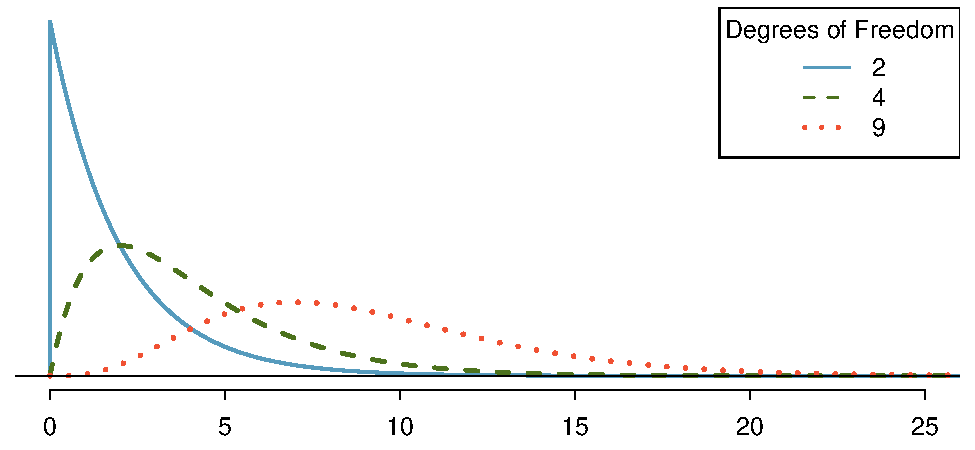
\includegraphics[width=0.9\textwidth]{ch_inference_for_props_oi_biostat/figures/chiSquareDistributionWithInceasingDF/chiSquareDistributionWithInceasingDF}
	\caption{Three chi-square distributions with varying degrees of freedom.}
	\label{chiSquareDistributionWithInceasingDF}
\end{figure}

\textD{\newpage}

The $\chi^2$ statistic from a contingency table has a sampling distribution that approximately follows a $\chi^2$ distribution with degrees of freedom $df = (r-1)(c-1)$, where $r$ is the number of rows and $c$ is the number of columns. Either statistical software or a table can be used to calculate $p$-values from the $\chi^2$ distribution. The \term{chi-square table} is partially shown in Figure~\ref{chiSquareProbabilityTableShort}, and a more complete table is presented in Appendix~\vref{chiSquareProbabilityTable}. This table is very similar to the $t$-table: each row provides values for distributions with different degrees of freedom, and a cut-off value is provided for specified tail areas. One important difference from the $t$-table is that the $\chi^2$ table only provides upper tail values.

\begin{figure}[h]
	\centering
	\begin{tabular}{r | rrrr | rrrr |}
		\hline
		Upper tail & 0.3 & 0.2 & 0.1 & 0.05 & 0.02 & 0.01 & 0.005 & 0.001 \\ 
		\hline
		df \hfill 1 & \footnotesize 1.07 & \footnotesize 1.64 & \footnotesize 2.71 & \footnotesize 3.84 & \footnotesize 5.41 & \footnotesize 6.63 & \footnotesize 7.88 & \footnotesize 10.83 \\ 
		\hfill 2 & \footnotesize 2.41 & \footnotesize 3.22 & \footnotesize 4.61 & \footnotesize 5.99 & \footnotesize 7.82 & \footnotesize 9.21 & \footnotesize 10.60 & \footnotesize 13.82 \\ 
		3 & \footnotesize 3.66 & \footnotesize 4.64 & \footnotesize 6.25 & \footnotesize 7.81 & \footnotesize 9.84 & \footnotesize 11.34 & \footnotesize 12.84 & \footnotesize 16.27 \\ 
		4 & \footnotesize 4.88 & \footnotesize 5.99 & \footnotesize 7.78 & \footnotesize 9.49 & \footnotesize 11.67 & \footnotesize 13.28 & \footnotesize 14.86 & \footnotesize 18.47 \\ 
		5 & \footnotesize 6.06 & \footnotesize 7.29 & \footnotesize 9.24 & \footnotesize 11.07 & \footnotesize 13.39 & \footnotesize 15.09 & \footnotesize 16.75 & \footnotesize 20.52 \\ 
		\hline
		6 & \footnotesize 7.23 & \footnotesize 8.56 & \footnotesize 10.64 & \footnotesize 12.59 & \footnotesize 15.03 & \footnotesize 16.81 & \footnotesize 18.55 & \footnotesize 22.46 \\ 
		7 & \footnotesize 8.38 & \footnotesize 9.80 & \footnotesize 12.02 & \footnotesize 14.07 & \footnotesize 16.62 & \footnotesize 18.48 & \footnotesize 20.28 & \footnotesize 24.32 \\ 
		\hline
	\end{tabular}
	\caption{A section of the chi-square table. A complete table is in Appendix~\vref{chiSquareProbabilityTable}.}
	\label{chiSquareProbabilityTableShort}
\end{figure}

\begin{examplewrap}
\begin{nexample}{Calculate an approximate $p$-value for the mammogram data, given that the $\chi^2$ statistic equals 0.02. Assess whether the data provides convincing evidence of an association between screening group and breast cancer death.}

The degrees of freedom in a $2 \times 2$ table is 1, so refer to the values in the first column of the probability table. The value 0.02 is less than 1.07, so the $p$-value is greater than 0.3. The data do not provide convincing evidence of an association between screening group and breast cancer death. This supports the conclusions from Example~\ref{mammogramExProp}, where the $p$-value was calculated to be 0.8650 and is visualized in Figure~\ref{mammogramPValue}.
\end{nexample}
\end{examplewrap}

\begin{figure}[h]
	\centering
	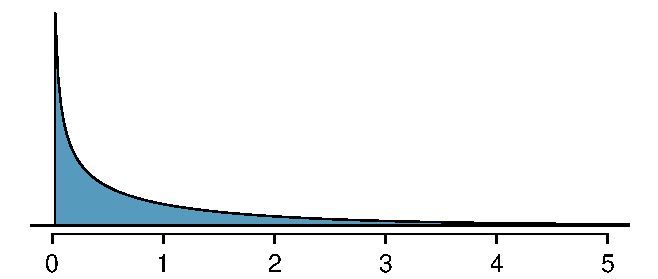
\includegraphics[width=0.6\textwidth]{ch_inference_for_props_oi_biostat/figures/mammogramPValue/mammogramPValue}
	\caption{The $p$-value for the mammogram data is shaded on the $\chi^2$ distribution with $df=1$.The shaded area is to the right of x = 0.02.}
	\label{mammogramPValue}
\end{figure}

\begin{exercisewrap}
\begin{nexercise}\label{hivDataPValue}%
Calculate an approximate $p$-value for the HIV data. Assess whether the data provides convincing evidence of an association between treatment and outcome at the $\alpha = 0.01$ significance level.\footnotemark{}
\end{nexercise}
\end{exercisewrap}
\footnotetext{The $\chi^2$ statistic is 14.7. For degrees of freedom 1, the tail area beyond 14.7 is smaller than 0.001. There is evidence to suggest that treatment is not independent of outcome.}


\textD{\newpage}


\subsection{Interpreting the results of a $\pmb{\chi^2}$ test}

If the $p$-value from a $\chi^2$ test is small enough to provide evidence to reject the null hypothesis of no association, it is important to explore the results further to understand direction of the observed association. This is done by examining the residuals, the standardized differences of the \emph{observed} - \emph{expected}, for each cell. Instead of using squared differences, the residuals are based on the differences themselves, and the standardizing or scaling factor is $\sqrt{\text{expected}}$.  Calculating residuals can be particularly helpful for understanding the results from large tables.

\index{residuals!contingency table}

For each cell in a table, the residual equals:
\[\dfrac{\text{observed} - \text{expected}}{\sqrt{\text{expected}}}. \]
Residuals with a large magnitude contribute the most to the $\chi^2$ statistic. If a residual is positive, the observed value is greater than the expected value, and vice versa for a negative residual.

\index{data!famuss|(}

\begin{examplewrap}
  \begin{nexample}
    {In the FAMuSS study introduced in Chapter~\ref{introductionToData}, researchers measured a variety of demographic and genetic characteristics for about 1,300 participants, including data on race and genotype at a specific locus on the ACTN3 gene (Figure~\ref{famussObservedCountsRaceGenotype}).
    Is there evidence of an association between genotype and race?} First, check the assumptions for applying a $\chi^2$ test. It is reasonable to assume independence, since it is unlikely that any participants were related to each other. None of the expected counts, as shown in Figure~\ref{famussExpectedRaceGenotype}, are less than 5.

$H_0$: Race and genotype are independent.

$H_A$: Race and genotype are not independent.

Let $\alpha = 0.05$.

Calculate the $\chi^2$ statistic:
\begin{align*}
\chi^2 &= \sum_{\text{all cells}} \frac{(\text{observed} - \text{expected})^2}{\text{expected}} \\
&= \dfrac{(16-7.85)^2}{7.85} + \dfrac{(6-11.84)^2}{11.84} + ... + \dfrac{(5 - 6.22)^2}{6.22} \\
&=19.4.
\end{align*}	

Calculate the $p$-value: for a table with 3 rows and 5 columns, the $\chi^2$ statistic is distributed with $(3-1)(5-1) = 8$ degrees of freedom. From the table, a $\chi^2$ value of 19.4 corresponds to a tail area between 0.01 and 0.02. Thus, there is sufficient evidence to reject the null hypothesis of independence between race and genotype.

The $p$-value can be obtained using the \textsf{R} function \texttt{pchisq} (\texttt{pchisq(19.4, df = 8, lower.tail = FALSE)}), which returns a value of 0.012861. %\footnote{\texttt{pchisq(19.4, df = 8, lower.tail = FALSE)}}

To further explore the differences in genotype distribution between races, calculate residuals for each cell (Figure~\ref{famussResidualsRaceGenotype}). The largest residuals are in the first row; there are many more African Americans with the CC genotype than expected under independence, and fewer with the CT genotype than expected. The residuals in the second row indicate a similar trend for Asians, but with a less pronounced difference. These results suggest further directions for research; a future study could enroll a larger number of African American and Asian participants to examine whether the observed trend holds with a more representative sample. Geneticists might also be interested in exploring whether this genetic difference between populations has an observable phenotypic \mbox{effect}.
\end{nexample}
\end{examplewrap}

% latex table generated in R 3.2.4 by xtable 1.8-2 package
% Wed Dec 07 22:13:57 2016
\begin{figure}[ht]
	\centering
	\begin{tabular}{r | l l l | l}
		\hline
		& CC & CT & TT & Sum \\ 
		\hline
		African American & 16 & 6 & 5 & 27 \\ 
		Asian & 21 & 18 & 16 & 55 \\ 
		Caucasian & 125 & 216 & 126 & 467 \\ 
		Hispanic & 4 & 10 & 9 & 23 \\ 
		Other & 7 & 11 & 5 & 23 \\ 
		\hline
		Sum & 173 & 261 & 161 & 595 \\ 
		\hline
	\end{tabular}
	\caption{Observed counts for race and genotype data from the FAMuSS study.}
    \label{famussObservedCountsRaceGenotype}
\end{figure}
%labels modified from xtable

% latex table generated in R 3.2.4 by xtable 1.8-2 package
% Thu Dec 08 10:34:51 2016
\begin{figure}[ht]
	\centering
	\begin{tabular}{r| l l l | l}
		\hline
		& CC & CT & TT & Sum \\ 
		\hline
		African Am & 7.85 & 11.84 & 7.31 & 27.00 \\ 
		Asian & 15.99 & 24.13 & 14.88 & 55.00 \\ 
		Caucasian & 135.78 & 204.85 & 126.36 & 467.00 \\ 
		Hispanic & 6.69 & 10.09 & 6.22 & 23.00 \\ 
		Other & 6.69 & 10.09 & 6.22 & 23.00 \\ 
		\hline
		Sum & 173.00 & 261.00 & 161.00 & 595.00 \\ 
		\hline
	\end{tabular}
	\caption{Expected counts for race and genotype data from the FAMuSS study.}
	\label{famussExpectedRaceGenotype}
\end{figure}
%labels and formatting modified

% latex table generated in R 3.2.4 by xtable 1.8-2 package
% Thu Dec 08 10:48:57 2016
\begin{figure}[ht]
	\centering
	\begin{tabular}{r|lll|l}
		\hline
		& CC & CT & TT & Sum \\ 
		\hline
		African Am & \highlightO{2.91} & \highlightO{-1.70} & -0.85 & 0.00 \\ 
		Asian & \highlightO{1.25} & \highlightO{-1.25} & 0.29 & 0.00 \\ 
		Caucasian & -0.93 & 0.78 & -0.03 & 0.00 \\ 
		Hispanic & -1.04 & -0.03 & 1.11 & 0.00 \\ 
		Other & 0.12 & 0.29 & -0.49 & 0.00 \\ 
		\hline
		Sum & 0.00 & 0.00 & 0.00 & 0.00 \\ 
		\hline
	\end{tabular}
	\caption{Residuals for race and genotype data from the FAMuSS study.}
     \label{famussResidualsRaceGenotype}
\end{figure}

\index{data!famuss|)}
\index{data!hiv}

\begin{examplewrap}
\begin{nexample}{In Guided Practice~\ref{hivDataPValue}, the $p$-value was found to be smaller than 0.001, suggesting that treatment is not independent of outcome. Does the evidence suggest that infants should be given nevirapine or lopinarvir?}\label{HIVDirectionEx}%

In a $2 \times 2$ table, it is relatively easy to directly compare observed and expected counts. 
For nevirapine, more infants than expected experienced virologic failure (60 > 44.6), while fewer than expected reached a stable disease state (87 < 102.4). For lopinarvir, fewer infants than expected experienced virologic failure (27 < 42.4), and more infants than expected reached a stable disease state (113 > 97.6) (Figure~\ref{observedAndExpectedCountsForTheHivStudy}). The outcomes for infants on lopinarvir are better than for those on nevirapine; combined with the results of the significance test, the data suggest that lopinarvir is associated with better treatment outcomes.
\end{nexample}
\end{examplewrap}

\begin{figure}[h]
	\centering
	\begin{tabular}{l | l l | l}
		\hline
		& NVP & LPV & Total \\
		\hline
		Virologic Failure & 60 \highlightO{44.6} & 27 \highlightO{42.4} & 87 \\
		Stable Disease & 87 \highlightO{102.4} & 113 \highlightO{97.6}& 200 \\	
		\hline
		Total & 147 & 140 & 287 \\
		\hline
	\end{tabular}
	\caption{Observed and \highlightO{(expected)} counts for the HIV study.}
	\label{observedAndExpectedCountsForTheHivStudy}
\end{figure}			
		
\begin{exercisewrap}
\begin{nexercise}
Confirm the conclusions reached in Example~\ref{HIVDirectionEx} by analyzing the residuals.\footnotemark{}
\end{nexercise}
\end{exercisewrap}
\footnotetext{$R_{1, 1} = \frac{(60 - 44.6)}{\sqrt{44.6}} = 2.31$; $R_{1, 2} = \frac{(27 - 42.4)}{\sqrt{42.4}} = -2.37$; $R_{2, 1} = \frac{(87-102.4)}{\sqrt{102.4}} = -1.53$; $R_{2, 2} = \frac{(113-97.6)}{\sqrt{97.6}} = 1.56$. The positive residuals for the upper left and lower right cells indicate that more infants than expected experienced virologic failure on NVP and stable disease on LPV; vice versa for the upper right and lower left cells. The larger magnitude of the residuals for the two NVP cells indicates that most of the discrepancy between observed and expected counts is for outcomes related to NVP.}

\index{data!LEAP}

\begin{exercisewrap}
\begin{nexercise}
Chapter~\ref{introductionToData} started with the discussion of a study examining whether exposure to peanut products reduce the rate of a child developing peanut allergies. Children were randomized either to the peanut avoidance or the peanut consumption group; at 5 years of age, each child was tested for peanut allergy using an oral food challenge (OFC). The results of the OFC are reproduced in Figure~\ref{leapStudyResultsTest}; failing the food challenge indicates an allergic reaction. Assess whether there is evidence for exposure to peanut allergy reducing the chance of developing peanut allergies.\footnotemark{}
\end{nexercise}
\end{exercisewrap}
\footnotetext{The assumptions for conducting a $\chi^2$ test are satisfied. Calculate a $\chi^2$ test statistic: 24.29. The associated $p$-value is $8.3 \times 10^{-7}$. There is evidence to suggest that treatment group is not independent of outcome. Specifically, a residual analysis shows that in the peanut avoidance group, more children than expected failed the OFC; in the peanut consumption group, more children than expected passed the OFC.}

% latex table generated in R 3.1.1 by xtable 1.7-4 package
% Thu Jul 16 07:12:04 2015
\begin{figure}[h]
	\centering
	\begin{tabular}{rrrr}
		\hline
		& FAIL OFC & PASS OFC & Sum \\ 
		\hline
		Peanut Avoidance & 36 & 227 & 263 \\ 
		Peanut Consumption & 5 & 262 & 267 \\ 
		Sum & 41 & 489 & 530 \\ 
		\hline
	\end{tabular}
	\caption{LEAP Study Results.} 
	\label{leapStudyResultsTest}
\end{figure}
%library(xtable); outcome.table = addmargins(table(LEAP$treatment.group, LEAP$overall.V60.outcome)); xtable(outcome.table, digits = 0, caption = "LEAP Study Results", caption  = "leapStudyResults")
	

\subsection{Fisher's exact test}
\label{fisherExactTest}

If sample sizes are too small, the $\chi^2$ distribution does not yield accurate $p$-values for  assessing  independence of the row and column variables in a table.  When expected counts in a table are less than 10, \term{Fisher's exact test} is often  used to calculate exact levels of significance. This test is usually applied to $2 \times 2$ tables. It can be applied to larger tables, but the logic behind the test is complex and the calculations involved are computationally intensive,  so this section covers only $2 \times 2$ tables. 

\index{data!fecal infusion|(}

\textit{Clostridium difficile} is a bacterium that causes inflammation of the colon. Antibiotic treatment is typically not effective, particularly for patients who experience multiple recurrences of infection. Infusion of feces from healthy donors has been reported as an effective treatment for recurrent infection. A randomized trial was conducted to compare the efficacy of donor-feces infusion versus vancomycin, the antibiotic typically prescribed to treat \textit{C. difficile }infection. The results of the trial are shown in Figure~\ref{fecalStudyResultsTest}.\footnote{These results correspond to the number of patients cured after the first infusion of donor feces and the number of patients cured in the vancomycin-alone group.} A brief calculation shows that all of the expected cell counts are less than 10, so the $\chi^2$ test should not be used as a test for association. 

Under the null hypothesis, the probabilities of cure in the fecal infusion and vancomycin groups are equal; i.e., individuals in one group are just as likely to be cured as individuals in the other group. Suppose the probability that an individual is cured, given that he or she was assigned to the fecal infusion group, is $p_1$ and the probability an individual is cured in the vancomycin group is $p_2$. Researchers were interested in testing the null hypothesis $H_0$: $p_1 = p_2$.

%data from \medicine\feces_infusion

\begin{figure}[h]
	\centering
	\begin{tabular}{rrrr}
		\hline
		& Cured & Uncured & Sum \\ 
		\hline
		Fecal Infusion & 13 & 3 & 16 \\ 
		Vancomycin & 4 & 9 & 13 \\ 
		Sum & 17 & 12 & 29 \\ 
		\hline
	\end{tabular}
	\caption{Fecal Infusion Study Results.} 
	\label{fecalStudyResultsTest}
\end{figure}

\textD{\newpage}

The $p$-value is the probability of observing results as or more extreme than those observed in the study under  the assumption that the null hypothesis is true. Previously discussed methods for significance testing have relied on calculating a test statistic associated with a defined sampling distribution, then obtaining $p$-values from tail areas on the distribution.  Fisher's exact test uses a similar approach, but introduces a new sampling distribution.  

The $p$-value for Fisher's exact test is calculated by adding together the individual conditional probabilities of obtaining each table that is as or more extreme than the one observed, under the null hypothesis and given that the marginal totals are considered fixed.

\begin{itemize}
	
	\item When the row and column totals are held constant, the value of any one cell in the table determines the rest of the entries. For example, if the marginal sums in Figure~\ref{fecalStudyResultsTest} are known, along with the value in one cell (e.g., the upper right equals 3), it is possible to calculate the values in the other three cells. Thus, when marginal totals are considered fixed, each table represents a unique set of results.
	
	\item Extreme tables are those which contradict the null hypothesis of $p_1 = p_2$. In the fecal infusion group, under the null hypothesis of no difference in the population proportion cured, one would expect $\frac{16 \times 17}{29} = 9.38$ cured individuals. The 13 observed cured individuals is extreme in the direction of more being cured than expected under the null hypothesis. An extreme result in the other direction would be, for instance, 1 cured patient in the fecal infusion group and 16 in the vancomycin group.
	
\end{itemize}

\begin{examplewrap}
\begin{nexample}{Of the 17 patients cured, 13 were in the fecal infusion group and 4 were in the vancomycin group. Assume that the marginal totals are fixed (i.e., 17 patients were cured, 12 were uncured, and 16 patients were in the fecal infusion group, while 13 were in the vancomycin group). Enumerate all possible sets of results that are more extreme than what was observed, in the same direction.}\label{fecalStudyExtreme}%
	
The observed results show a case of $\hat{p}_1 > \hat{p}_2$; results that are more extreme consist of cases where more than 13 cured patients were in the fecal infusion group. Under the assumption that the total number of cured patients is constant at 17 and that only 16 patients were assigned to the fecal infusion group (out of 29 patients total), more extreme results are represented by cases where 14, 15, or 16 cured patients were in the fecal infusion group. The following tables illustrate the unique combinations of values for the 4 table cells corresponding to those extreme results.

\begin{center}
	\color{gray}
	\begin{tabular}{r|cc|c}
		\hline
		& Cured & Uncured & Sum \\ 
		\hline
		Fecal Infusion & \textcolor{black}{14} & \textcolor{black}{2} & 16 \\ 
		Vancomycin & \textcolor{black}{3} & \textcolor{black}{10} & 13 \\ 
		\hline
		Sum & 17 & 12 & 29 \\ 
		\hline
	\end{tabular}

	\color{gray}
	\begin{tabular}{r|cc|c}
		\hline
		& Cured & Uncured & Sum \\ 
		\hline
		Fecal Infusion & \textcolor{black}{15} & \textcolor{black}{1} & 16 \\ 
		Vancomycin & \textcolor{black}{2} & \textcolor{black}{11} & 13 \\ 
		\hline
		Sum & 17 & 12 & 29 \\ 
		\hline
	\end{tabular}

	\color{gray}
	\begin{tabular}{r|cc|c}
		\hline
		& Cured & Uncured & Sum \\ 
		\hline
		Fecal Infusion & \textcolor{black}{16} & \textcolor{black}{0} & 16 \\ 
		Vancomycin & \textcolor{black}{1} & \textcolor{black}{12} & 13 \\ 
		\hline
		Sum & 17 & 12 & 29 \\ 
		\hline
	\end{tabular}
\end{center}
\end{nexample}
\end{examplewrap}


\subsubsection{Calculating a one-sided $\pmb{\MakeLowercase{p}}$-value}

Suppose that researchers were interested in testing the null hypothesis against the one-sided alternative, $H_A: p_1 > p_2$. To calculate the one-sided $p$-value, sum the probabilities of each table representing results as or more extreme than those observed; specifically, sum the probabilities of observing Figure~\ref{fecalStudyResultsTest} and the tables in Example~\ref{fecalStudyExtreme}.

\begin{figure}[h]
	\centering
	\begin{tabular}{rccc}
		\hline
		& Cured & Uncured & Sum \\ 
		\hline
		Fecal Infusion & $a$ & $b$ & $a+b$ \\ 
		Vancomycin & $c$ & $d$ & $c+d$ \\ 
		Sum & $a+c$ & $b+d$ & $n$ \\ 
		\hline
	\end{tabular}
	\caption{General Layout of Data in Fecal Infusion Study.} 
	\label{fecalStudyGeneral}
\end{figure}

The probability of observing a table with cells $a, b, c, d$ given fixed marginal totals $a+b$, $c+d$, $a + c$, and $b +d$ follows the hypergeometric distribution.  The hypergeometric distribution was introduced in Section~\ref{hypergeometric}.

\[P(a,b,c,d) = \text{HGeom}(a+b, c+d, a+c) = \dfrac{ {a+b \choose a} {c+d \choose c}}{{n \choose a+c}} = \dfrac{(a+b)! \text{ } (c+d)! \text{ } (a+c)! \text{ } (b+d)!}{a! \text{ } b! \text{ } c! \text{ } d! \text{ } n!}.\]

\begin{examplewrap}
\begin{nexample}{Calculate the probability of observing Figure~\ref{fecalStudyResultsTest}, assuming the margin totals are fixed.}

\[P(13, 3, 4, 9) = \dfrac{ {16 \choose 13} {13 \choose 4}}{{29 \choose 17}} = \dfrac{16! \text{ } 13! \text{ } 17! \text{ } 12!}{13! \text{ } 3! \text{ } 4! \text{ } 9! \text{ } 29!} = 7.71 \times 10^{-3}.\]

The value 0.0077 represents the probability of observing 13 cured patients out of 16 individuals in the fecal infusion group and 1 cured in the vancomycin group, given that there are a total of 29 patients and 17 were cured overall.
\end{nexample}
\end{examplewrap}

\begin{examplewrap}
\begin{nexample}{Evaluate the statistical significance of the observed data in Figure~\ref{fecalStudyResultsTest} using the one-sided alternative $H_A: p_1 > p_2$.}

Calculate the probability of the tables from Example~\ref{fecalStudyExtreme}. Generally, the formula for these tables is 
\[P(a, b, c, d) = \dfrac{ {a+b \choose a} {c+d \choose c}}{{n \choose a+c}} = \dfrac{ {16 \choose a} {13 \choose c}}{{29 \choose 17}},\] 
since the marginal totals from Figure~\ref{fecalStudyResultsTest} are fixed. The value $a$ ranges from 14, 15, 16, while $c$ ranges from 3, 2, 1.
\begin{align*}
P(14, 2, 3, 10) &= \dfrac{ {16 \choose 14} {13 \choose 3}}{{29 \choose 17}} = 6.61 \times 10^{-4} \\
P(15, 1, 2, 11) &= \dfrac{ {16 \choose 15} {13 \choose 2}}{{29 \choose 17}} = 2.40 \times 10^{-5} \\
P(16, 0, 1, 12) &= \dfrac{ {16 \choose 16} {13 \choose 1}}{{29 \choose 17}} = 2.51 \times 10^{-7}
\end{align*}

The probability of the observed table is $7.71 \times 10^{-3}$, as calculated in the previous example.

The one-sided $p$-value is the sum of these table probabilities: $(7.71 \times 10^{-3}) + (6.61 \times 10^{-4}) + (2.40 \times 10^{-5}) + (2.51 \times 10^{-7}) = 0.0084.$

The results are significant at the $\alpha = 0.05$ significance level. There is evidence to support the one-sided alternative that the proportion of cured patients in the fecal infusion group is higher than the proportion of cured patients in the vancomycin group. However, it is important to note that two-sided alternatives are the standard in medical literature. Conducting a two-sided test would be especially desirable when evaluating a treatment which lacks randomized trials supporting its efficacy, such as donor-feces infusion.
\end{nexample}
\end{examplewrap}


\subsubsection{Calculating a two-sided $\pmb{\MakeLowercase{p}}$-value}

There are various methods for calculating a two-sided $p$-value in the Fisher's exact test setting. When the test is calculated by hand, the most common way to calculate a two-sided $p$-value is to double the smaller of the one-sided $p$-values. One other common method used by various statistical computing packages such as \textsf{R} is to classify "more extreme" tables as all tables with probabilities less than that of the observed table, in both directions. The two-sided $p$-value is the sum of probabilities for the qualifying tables.  That approach is illustrated in the next example.

\begin{examplewrap}
\begin{nexample}{Evaluate the statistical significance of the observed data in Figure~\ref{fecalStudyResultsTest} using the two-sided alternative $H_A: p_1 \neq p_2$.}
	
Identify tables that are more extreme in the other direction of the observed result, i.e. where the proportion of cured patients in the vancomycin group are higher than in the fecal infusion group. Start with the most extreme cases and calculate probabilities until a table has a $p$-value higher than $7.71 \times 10^{-3}$, the probability of the observed table. 

The most extreme result in the $\hat{p}_1 < \hat{p}_2$ direction would be if all patients in the vancomycin group were cured; then 13 of the cured patients would be in the vancomycin group and 4 would be in the fecal transplant group. This table has probability $3.5 \times 10^{-5}$.

\begin{center}
	\color{gray}
	\begin{tabular}{r|cc|c}
		\hline
		& Cured & Uncured & Sum \\ 
		\hline
		Fecal Infusion & \textcolor{black}{4} & \textcolor{black}{12} & 16 \\ 
		Vancomycin & \textcolor{black}{13} & \textcolor{black}{0} & 13 \\ 
		\hline
		Sum & 17 & 12 & 29 \\ 
		\hline
	\end{tabular}
\end{center}

Continue enumerating tables by decreasing the number of cured patients in the vancomycin group. The table with 5 cured patients in the fecal infusion group has probability $1.09 \times 10^{-3}$.

\begin{center}
	\color{gray}
	\begin{tabular}{r|cc|c}
		\hline
		& Cured & Uncured & Sum \\ 
		\hline
		Fecal Infusion & \textcolor{black}{5} & \textcolor{black}{11} & 16 \\ 
		Vancomycin & \textcolor{black}{12} & \textcolor{black}{1} & 13 \\ 
		\hline
		Sum & 17 & 12 & 29 \\ 
		\hline
	\end{tabular}
\end{center}

The table with 6 cured patients in the fecal infusion group has probability 0.012. This value is greater than $7.71 \times 10^{-3}$, so it will not be part of the sum to calculate the two-sided $p$-value.
	
\begin{center}
	\color{gray}
	\begin{tabular}{r|cc|c}
		\hline
		& Cured & Uncured & Sum \\ 
		\hline
		Fecal Infusion & \textcolor{black}{6} & \textcolor{black}{10} & 16 \\ 
		Vancomycin & \textcolor{black}{11} & \textcolor{black}{2} & 13 \\ 
		\hline
		Sum & 17 & 12 & 29 \\ 
		\hline
	\end{tabular}
\end{center}

As calculated in the previous example, the one-sided $p$-value is $0.0084$. Thus, the two-sided $p$-value for these data equals $0.0084 + (3.5 \times 10^{-5}) + (1.09 \times 10^{-3}) = 0.0095$. The results are significant at the $\alpha = 0.01$ significance level, and there is evidence to support the efficacy of donor-feces infusion as a treatment for recurrent \textit{C. difficile} infection.
\end{nexample}
\end{examplewrap}

\index{data!fecal infusion|)}


%__________________
\section[Chi-square tests for the fit of a distribution]{Chi-square tests for the fit of a distribution}
\label{oneWayChiSquare}

The $\chi^2$ test can also be used to examine the appropriateness of hypothesized distribution for a dataset, most commonly when a set of observations falls naturally into categories as in the examples discussed in this section. As with testing in the two-way table setting, expected counts are calculated based on the assumption that the hypothesized distribution is correct, and the statistic is based on the discrepancies between observed and expected counts. The  $\chi^2$ sampling distribution for the test statistic is reasonably accurate when each expected count is at least 5 and follows a $\chi^2$ distribution with $k-1$ degrees of freedom, where $k$ is the number of categories.  Some guidelines recommend that no more than 1/5 of the cells have expected counts less than 5, but the stricter requirement that all cells have expected counts greater than 5 is safer.

When used in this setting, the $\chi^2$ test is often called a \termsub{`goodness-of-fit' test}{goodness-of-fit test}, a term that is often misunderstood.  Small $p$-values of the test suggest evidence that a hypothesized distribution is not a good model, but non-significant $p$-values do not imply that the hypothesized distribution is the best model for the data, or even a good one. In the logic of hypothesis testing, failure to reject a null hypothesis cannot be viewed as evidence that the null hypothesis is true.

\index{data!famuss|(}

\begin{examplewrap}
\begin{nexample}{The participants in the FAMuSS study were volunteers at a university, and so did not come from a random sample of the US population.  The participants may not be representative of the general United States population. The $\chi^2$ test can be used to test the null hypothesis that the participants are racially representative of the general population. Figure~\ref{famussRacialProportions} shows the number observed by racial category in FAMuSS and the proportions of the US population in each of those categories.\footnotemark{}}

Under the null hypothesis, the sample proportions should equal the population proportions. For example, since African Americans are 0.128 of the general proportion, $(0.128)(595) = 76.16$ African Americans would be expected in the sample.  The rest of the expected counts are shown in Figure~\ref{actualExpectedRacialCountsFamuss}.

Since each expected count is greater than or equal to 5,  the $\chi^2$ distribution can be used to calculate a $p$-value for the test.

\begin{align*}
\chi^2 &= \sum_{\text{all cells}} \frac{(\text{observed} - \text{expected})^2}{\text{expected}} \\
&= \dfrac{(27-76.16)^2}{76.16} + \dfrac{(55-5.95)^2}{5.95} + \dfrac{(467-478.38)^2}{478.38} + \dfrac{(46-34.51)^2}{34.51} \\
&=440.18.
\end{align*}	

There are 3 degrees of freedom, since $k = 4$. The $\chi^2$ statistic is extremely large, and the associated tail area is smaller than 0.001. There is more than sufficient evidence to reject the null hypothesis that the sample is representative of the general population. A comparison of the observed and expected values (or the residuals) indicates that the largest discrepancy is with the over-representation of Asian participants.
\end{nexample}
\end{examplewrap}
\footnotetext{The US Census Bureau considers Hispanic as a classification separate from race, on the basis that Hispanic individuals can be any race. In order to facilitate the comparison with the FAMuSS data, participants identified as "Hispanic" have been merged with the "Other" category.}

\textD{\newpage}

\begin{figure}[h]
	\centering
	\begin{tabular}{ll ccc c ll}
		\hline
		Race	 & \hspace{2mm} & African American & Asian & Caucasian & Other & \hspace{2mm} & Total \\
		\hline
		FAMuSS &	& 27 & 55 & 467 & 46 & & 595 \\
		US Census	 & 		& 0.128 & 0.01 & 0.804 & 0.058 & & 1.00 \\
		\hline
	\end{tabular}
	\caption{Representation by race in the FAMuSS study versus the general population.}
    \label{famussRacialProportions}
\end{figure}

\begin{figure}[h]
	\centering
	\begin{tabular}{ll ccc c ll}
		\hline
		Race	 & \hspace{2mm} & African American & Asian & Caucasian & Other & \hspace{2mm} & Total \\
		\hline
		Observed &	& 27 & 55 & 467 & 46 & & 595 \\
		Expected & 	& 76.16 & 5.95 & 478.38 & 34.51 & & 595 \\
		\hline
	\end{tabular}
	\caption{Actual and expected counts in the FAMuSS data.}
    \label{actualExpectedRacialCountsFamuss}
\end{figure}	

\index{data!famuss|)}
%2004 US Census data: https://www.census.gov/population/pop-profile/dynamic/RACEHO.pdf

\index{data!Arabidopsis thaliana}

\begin{examplewrap}
\begin{nexample}{According to Mendelian genetics, alleles segregate independently; if an individual is heterozygous for a gene and has alleles $A$ and $B$, then the alleles have an equal chance of being passed to an offspring. Under this framework, if two individuals with genotype $AB$ mate, then their offspring are expected to exhibit a 1:2:1 genotypic ratio; 25\% of the offspring will be $AA$, 50\% will be $AB$, and 50\% will be $BB$. The term "segregation distortion" refers to a deviation from expected Mendelian frequencies. 
		
At a specific gene locus in the plant \textit{Arabidopsis thaliana}, researchers have observed 84 $AA$ individuals, 233 $AB$ individuals, and 134 $BB$ individuals. Is there evidence of segregation disorder at this locus? Conduct the test at $\alpha = 0.0001$ to account for multiple testing, since the original study examined approximately 250 locations across the genome.}

The Mendelian proportions are 25\%, 50\%, and 25\%. Thus, the expected counts in a group of 451 individuals are: 112.75 $AA$, 225.50 $AB$, and 112.75 $BB$. No expected count is less than 5.

\begin{align*}
\chi^2 &= \sum_{\text{all cells}} \frac{(\text{observed} - \text{expected})^2}{\text{expected}} \\
&= \dfrac{(84-112.75)^2}{112.75} + \dfrac{(233-225.50)^2}{225.50} + \dfrac{(134-112.75)^2}{112.75}\\
&=11.59.
\end{align*}
There are 2 degrees of freedom, since $k = 3$. The $p$-value is between 0.005 and 0.001, which is greater than $\alpha = 0.0001$. There is insufficient evidence to reject the null hypothesis that the offspring ratios correspond to expected Mendelian frequencies; i.e., there is not evidence of segregation distortion at this locus.
\end{nexample}
\end{examplewrap}


%___________
\section{Outcome-based sampling: case-control studies}
\label{caseControlStudies}

\index{case-control studies|(}

\subsection{Introduction}

The techniques so far in this chapter have often relied on the assumption that the data were collected using random sampling from a population.  When cases come from a random sample, the sample proportion of observations with a particular outcome should accurately estimate the population proportion, given that the sample size is large enough.  When studying rare outcomes, however, moderate sized samples may contain few or none of the outcomes.  Persistent pulmonary hypertension of the newborn (PPHN) is a dangerous condition in which the blood vessels in the lungs of a newborn do not relax immediately after birth, leading to inadequate oxygenation.   The condition is rare, occurring in about 1.9 per 1,000 live births, so it is difficult to study using random sampling.  In the early 2000s, anecdotal evidence began to accumulate that the risk of the condition might be increased if the mother of the newborn had been taking a particular medication for depression, a selective serotonin reuptake inhibitor (SSRI) during the third trimester of pregnancy or even as early as during week 20 of the pregnancy.  

One design for studying the issue would enroll two cohorts of women, one in which women were taking SSRIs for depression and one in which they were not. However, if the chance of PPHN was 1.9/1,000 in newborns of a control cohort of 1,000 women, then the probability of observing no cases of PPHN is about 0.15. If the probability of PPHN is elevated among infants born to women taking SSRIs, such as to 3.0/1,000, the chance of observing no cases among 1,000 women is approximately 0.05. Precise measures of the probability of PPHN occurring would require very large cohorts.

\index{sample!outcome-dependent}

An alternative design for studies like this reverses the sampling scheme so that the two cohorts are determined by outcome, rather than exposure; a cohort with the condition and a cohort without the condition are sampled, then exposure to a possible cause is recorded. To apply this design for studying PPHN, a registry of live births could be used to sort births by presence or absence of PPHN. The number in each group in which the mother had been taking SSRIs could then be recorded (based on medical records). Such a design would have the advantage of sufficient numbers of cases with and without PPHN, but it has other limitations which will be discussed later in this section. Traditionally, these studies have been called case-control studies because of the original sampling of individuals with and without a condition.  More generally, it is an example of outcome-dependent sampling.


\textD{\newpage}


\subsection{$\pmb{\chi^2}$ tests of association in case-control studies}
\label{caseControlTests}

\index{case-control studies!tests for association}
\index{data!persistent pulmonary hypertension in newborns (PPHN)|(}

In 2006, Chambers, et. al reported a case-control study examining the association of SSRI use and persistent pulmonary hypertension in newborns.\footnote{N Engl J Med 2006;354:579-87.}  The study team enrolled 337 women whose infants suffered from PPHN and 836 women with similar characteristics but whose infants did not have PPHN.  Among the women whose infants had PPHN, 14 had taken an SSRI after week 20 of the pregnancy.  In the cohort of women whose infants did not have PPHN, 6 had been taking the medication after week 20. In the subset of women who had been taking an SSRI, the infants are considered `exposed' to the medication. The data from the study are summarized in Figure~\ref{ssriPPHNObserved}.

\begin{figure}[h]
	\centering
	\begin{tabular}{ll rrr r}
		\hline
		PPHN present	 & \hspace{2mm} & Yes & No & \hspace{2mm} & Total \\
		\hline
		SSRI exposed &	& 14 & 6 &  & 20  \\
		SSRI unexposed & & 323 & 830 &  & 1153  \\
        Total & & 337 & 836 & & 1173 \\
		\hline
	\end{tabular}
	\caption{SSRI exposure vs observed number of PPHN cases in newborns.}
    \label{ssriPPHNObserved}
\end{figure}	

The sample of women participating in the study are clearly not a random sample drawn from women who had recently given birth; they were identified according to the disease status of their infants.  In this sample, the proportion of newborns with PPHN (337/1173 = 28.7\%) is much higher than the disease prevalence in the general population.  

Even so, the concept of independence between rows and columns under a null hypothesis of no association still holds. If SSRI use had no effect on the occurrence of PPHN, then the proportions of mothers taking SSRIs among the PPHN and non-PPHN infants should be about the same. In other words, the null hypothesis of equal SSRI use among mothers with/without PPHN affected infants is the hypothesis of no association between SSRI use and PPHN. The test of independence can be conducted using the approach introduced earlier in the chapter.

The expected counts shown in Figure~\ref{ssriPPHNExpected} suggest that the $p$-value from a $\chi^2$ test may not be accurate; under the null hypothesis, the expected number of PPHN cases in the SSRI exposed group is less than 10.

 \begin{figure}[h]
	\centering
	\begin{tabular}{ll rrr r}
		\hline
		PPHN present  & \hspace{2mm} & Yes & No & \hspace{2mm} & Total \\
		\hline
		SSRI exposed &	& 5.80 & 14.20 &  & 20  \\
		SSRI unexposed & & 331.20 & 811.80 &  & 1153  \\
        Total & & 337 & 836 & & 1173 \\
		\hline
	\end{tabular}
    \caption{SSRI exposure vs expected number of PPHN cases in newborn.}
    \label{ssriPPHNExpected}
\end{figure}	

The $p$-value from Fisher's exact test is $< 0.001$ ($0.00014$, to be precise), so the evidence is strong that SSRI exposure and PPHN are associated. Fisher's exact test is often used in studies of rare conditions or exposures since one or more expected cell counts are typically less than 10.

\index{data!persistent pulmonary hypertension in newborns (PPHN)|)}


\textD{\newpage}


\subsection{Estimates of association in case-control studies}
\label{caseControlStudiesEstimates}

\index{odds ratio!case-control studies}

For data in a $2 \times 2$ table, correct point estimates of association depend on the mechanism used to gather the data.  In the example of a clinical trial of nevirapine versus lopinarvir discussed in Section~\ref{twoWayTablesExpectedCounts}, the population proportion of children who would experience virologic failure after treatment with one of the drugs can be estimated by the observed proportion of virologic failures while on that drug. For nevirapine, the proportion of children with virologic failure is 60/147 = 0.41, while for lopinarvir the proportion is 27/140 = 0.19.  The difference in outcome between the two groups can be summarized by the difference in these proportions. The proportion experiencing virologic failure when treated with nevirapine was 0.12 larger in nevirapine (0.41 - 0.29), so if the two drugs were to be used in a large population, approximately 12\% more children treated with nevirapine would experience virologic failure as compared to lopinarvir. The confidence intervals discussed in Section~\ref{confidenceIntervalsDifferenceProportions} can be used to express the uncertainty in this estimate.

Since the proportion of virologic failures can be estimated from the trial data, the relative risk of virologic failure can also be used to estimate the association between treatment and virologic failure. Relative risk is the ratio of two proportions, and was introduced in Section~\ref{TwoWayTablesRelativeRisk}.  The relative risk of virologic failure with nevirapine versus lopinarvir is $0.41/0.19 = 2.16$.  Children treated with nevirapine are estimated to be more than twice as likely to experience virologic failure.  

Statistically, the population parameter for the relative risk in the study of HIV$^+$ is a ratio of conditional probabilities:

\begin{align*}
  \frac{P(\text{virologic failure}| \text{treatment with nevirapine})}
  {P(\text{virologic failure}|\text{treatment with lopinarvir})}.
\end{align*}

In a study like the PPHN case-control study, the natural population parameter of interest would be the relative risk of PPHN for infants exposed to an SSRI during after week 20 of gestation compared to those who were not exposed. However, in the design of this study, participating mothers were sampled and grouped according to whether their infants did or did not suffer from PPHN, rather than assigned to either SSRI exposure or non-exposure. Relative risk of PPHN from exposure to SSRI cannot be estimated from the data because it is not possible to estimate $P(\text{PPHN} | \text{SSRI exposure})$ and $P(\text{PPHN} | \text{no SSRI exposure})$. In case-control studies, association is estimated using \term{odds} and \termsub{odds ratios}{odds ratio} rather than relative risk.

The \term{odds} of SSRI exposure among the cases are given by the fraction
\[
  \text{odds$_\text{cases}$} = \frac{P(\text{SSRI exposure} | \text{PPHN})}
  {P(\text{no SSRI exposure} | \text{PPHN})} = \frac{14/337}{323/337} = \frac{14}{323}.
\]

The odds of SSRI exposure among the controls are given by the fraction
\[
  \text{odds$_\text{controls}$} = \frac{P(\text{SSRI exposure} | \text{no PPHN})}
  {P(\text{no SSRI exposure} | \text{no PPHN})} = \frac{6/836}{830/836} = \frac{6}{830}.
\]

The ratio of the odds, the odds ratio, compares the odds of exposure among the cases to the odds of exposure among the controls: 

\[OR_{\text{exposure, cases vs. controls}} = \frac{\text{odds$_\text{cases}$}}{\text{odds$_\text{controls}$}} = \frac{14/323}{6/830} = \frac{(14)(830)}{(323)(6)} =  6.00. \]

\textD{\newpage}

A population odds ratio of, for example, 1.5, implies that the odds of exposure in cases are 50\% larger than the odds of exposure in controls. For this study, the odds ratio of 6.00 implies that the odds of SSRI exposure in infants with PPHN are 6 times as large as the odds of exposure in infants without PPHN. Epidemiologists describe this odds ratio as the odds of exposure given presence of PPHN compared to the odds of exposure given absence of PPHN. An OR greater than 1 suggests that the exposure may be a risk factor for the disease or condition under study.  Epidemiologists also use the term \term{relative odds} as a synonym for odds ratio.

Surprisingly, the odds ratio of exposure comparing cases to controls is equivalent to the odds ratio of disease comparing exposed to unexposed.\footnote{This result can be shown through Bayes' rule.} With a specific example, it is easy to see how the fraction for the odds ratios are numerically equivalent:

\[OR_{\text{disease, exposed versus unexposed}} = \frac{\text{odds$_\text{exposed}$}}{\text{odds$_\text{unexposed}$}} = \frac{14/6}{323/830} = \frac{(14)(830)}{(6)(323)} = 6.00. \]

Despite the apparently restrictive nature of the case-control sampling design, the odds ratio of interest, the odds ratio for disease given exposure, can be estimated from case-control data.

Epidemiologists rely on one additional result, called the rare disease assumption. When a disease is rare, the odds ratio for the disease given exposure is approximately equal to the relative risk of the disease given exposure.  These identities are the reason case-control studies are widely used in settings in which a disease is rare: it allows for the relative risk of disease given exposure to be estimated, even if the study design is based on sampling cases and controls then measuring exposure.

In a general $2 \times 2$ table of exposure versus disease status (Figure~\ref{generalTwoByTwoTable}) the odds ratio for disease given exposure status is the $ad/bc$.
 \begin{figure}[h]
	\centering
	\begin{tabular}{ll rrr r}
		\hline
		Disease Status  & \hspace{2mm} & Present & Absent & \hspace{2mm} & Total \\
		\hline
		Exposed &	& $a$ & $b$ &  & $a + b$  \\
		Unexposed & & $c$ & $d$ &  & $c + d $  \\
        Total & & $a + c$ & $b + d$ & & $n$ \\
		\hline
	\end{tabular}
    \caption{Exposure vs Disease Status.}
    \label{generalTwoByTwoTable}
\end{figure}

In the PPHN case-control data, the odds ratio for PPHN given SSRI exposure status is $(14)(830)/(6)(323) = 6.00$.  Because PPHN is a rare condition, the risk of PPHN among infants exposed to an SSRI is estimated to be approximately 6 times that of the risk among unexposed infants.  Infants exposed to an SSRI are 600\% more likely to suffer from PPHN.

It can be shown that the $p$-value used in a test of no association (between exposure and disease) is also the $p$-value for a test of the null hypothesis that the odds ratio is 1.

\index{case-control studies|)}

\section{Inference for two samples of binary data} \label{inferenceBinaryData}

\noindent{ \textit{NOTE: This supplement to the first edition is being released online as an extension to Chapter 8. Its pagination corresponds to the printed first edition text. This supplement includes a set of exercises and solutions to the odd-numbered exercises.}}

\vspace{0.5cm}

Methods for summarizing data from two samples of binary data were introduced in  Sections~\ref{twoCategoricalVariables} and \ref{caseControlStudies}, where relative risk and odds ratios were introduced.  Methods for inference for the difference of two proportions were discussed in Sections~\ref{differenceOfTwoProportions} and \ref{twoWayTablesAndChiSquare}.  This supplement provides more details about those measures when used to compare two groups, adding information about terminology, interpretation, hypothesis tests, and confidence intervals for relative risk and odds ratios.  For convenience, some of the earlier material on inference for the difference in two proportions is reviewed in this supplement.

%____________________

\subsection{Introduction and terminology}
\label{introAndTerminologyForRisk}

This section reviews concepts and terminology for summary measures of association in two groups (e.g., an intervention or exposure) when the outcome has two values (e.g., yes/no, success/failure, or 0/1).  The ideas summarized here are discussed in more detail in later sections.


\subsubsection{Risk ratio (relative risk) and risk difference}

The term risk is often used in statistics and epidemiology as the likelihood of a condition or an outcome from a disease, such as the risk of diabetes among young adults or the risk of Covid-19 infection in a particular population. Since prevalence is a better term for the likelihood of a condition in a population,  this section limits the term risk to settings in which the potential causal effect of an intervention or exposure is examined, such as a study examining whether a new treatment for Covid-19 reduces the risk of severe disease in a cohort of infected individuals. A causal effect can be estimated only in studies where an outcome is measured after a study participant has received an intervention or experienced an exposure. Randomized experiments are the best designs for estimating a potential causal effect since they reduce the chance of confounding, but risk can also be suggested by some observational studies, so the term risk is used here more widely than for just randomized experiments.

 In the LEAP study discussed in the first section of Chapter~\ref{introductionToData} the study team investigated whether an intervention beginning in infancy would reduce the risk  of a child developing a peanut allergy by age 5 years. Of the 263 children randomized to the peanut avoidance group, 36 showed signs of a peanut allergy at 5 years of age.  The estimated risk of an allergy is 36/263 = 0.137.  Five of the 267 assigned to the peanut consumption group experienced signs of an allergy, for an estimated risk of 5/267 = 0.019. The estimated risk ratio (also called relative risk)\footnote{The term relative risk is more common than risk ratio, but the latter is more descriptive and is used in this section.} of developing an allergy, comparing the avoidance to the consumption group, is 0.137/0.019 = 7.21.  Children in the avoidance group were more than 7 times as likely to develop an allergy compared to those in the consumption group.

The estimated risk difference in the LEAP study is 0.137 - 0.019 = 0.118.  On an additive scale, the risk of a peanut allergy increases by slightly more than 0.10 (10\%) for children in the avoidance group.  Risk ratios and differences provide important summary statistics when comparing groups, but in some settings one is more informative than the other.  When overall risk is small, as is the case with peanut allergies, risk ratios are often more informative.  A small risk difference of 0.118 is associated with a large multiplicative increase in the probability of outcome. When overall risk is larger, a risk ratio may potentially obscure the magnitude of an effect. For example, suppose overall risk is 0.40 and an intervention under study is thought to reduce risk to 0.35. In a large population, this reduction in absolute risk of 0.05 may be clinically relevant; in a population of 1,000,000 a reduction in risk from 0.40 to 0.35 will reduce the occurrence of the condition from 400,000 to 350,000, affecting 50,000 individuals. The relative risk of 0.40/0.35 = 1.14 does not convey the same message as the risk difference. Whichever summary statistic is used as the primary measure of comparison, both should be provided in the interpretation of a study.

The calculation of risk ratio in the LEAP study used the peanut consumption group as the baseline.  The risk in the peanut avoidance group could have been used for the baseline, yielding a relative risk of 0.019/0.137 = 0.139.  This risk of allergy in the consumption group is approximately 0.14 times that of avoidance group.  While there is no set convention for the choice of the baseline group, risk ratios greater than 1 are easier for most people to interpret so the baseline group is usually chosen to be the one with the smaller risk.

\subsubsection{Prevalence ratio and prevalence difference}

The calculations for prevalence ratios and differences mirror those for risk ratios and differences, but the different terminology reflects an important difference in interpretation.  The prevalence of a disease is the proportion of a population experiencing the disease.  Cross-sectional studies sample a population during a prespecified (usually short) time interval and can be used to estimate the prevalence of a disease and features of the population that may be associated with the disease. Since a cross-sectional study does not measure an outcome occurring subsequent to an exposure, it cannot estimate risk of an outcome from an exposure.  Cross-sectional studies can, however, provide important information about the association between outcome and features of a population that might justify additional studies.

The US CDC estimates that approximately 14.9\% of non-Hispanic Asian adults in the United States have Type 2 diabetes (T2D);\footnote{Centers for Disease Control and Prevention. National Diabetes Statistics Report, 2020.}  the prevalence of T2D in this population is 0.149.  For non-Hispanic white adults, the prevalence of T2D is 0.119 (11.9\%). The prevalence difference between the groups, comparing non-Hispanic Asian to non-Hispanic white adults, is 0.149 - 0.119 = 0.03.  The prevalence ratio comparing Asian to white non-Hispanics is 0.149/0.119 = 1.252.  The prevalence of T2D for Asian adults is 1.252 times as large as that for white adults.

\subsubsection{Odds ratios}

Odds ratios are used to estimate an association between an outcome and exposure when baseline risk or prevalence cannot be estimated, such as in a case-control study. In a dataset, the observed odds of an event is the number of times the event happens divided by the number of times it does not.  The odds ratio (OR) is the odds of an event occurring in one group divided by the odds of an event occurring in the baseline group.  Somewhat surprisingly, even when risk or prevalence ratio cannot be estimated, the OR comparing the odds of an outcome between exposed and unexposed groups can.

Figure~\ref{ssriPPHNObserved} in Section~\ref{caseControlStudies} summarizes the results of a study examining the association of persistent pulmonary hypertension of a newborn (PPHN) with exposure to maternal use of a selective serotonin re-uptake inhibitor (SSRI) during pregnancy. For convenience, the figure is repeated here as Figure~\ref{ssriPPHNObservedRepeated}.

\begin{figure}[h]
	\centering
	\begin{tabular}{ll rrr r}
		\hline
		PPHN present	 & \hspace{2mm} & Yes & No & \hspace{2mm} & Total \\
		\hline
		SSRI exposed &	& 14 & 6 &  & 20  \\
		SSRI unexposed & & 323 & 830 &  & 1153  \\
        Total & & 337 & 836 & & 1173 \\
		\hline
	\end{tabular}
	\caption{SSRI exposure versus observed number of PPHN cases in newborns.}
    \label{ssriPPHNObservedRepeated}
\end{figure}

Participants in the PPHN study were sampled and grouped according to whether their infants did or did not suffer from PPHN; the study did not count the number of PPHN outcomes among women using an SSRI during pregnancy. Thus, the absolute risk of PPHN given SSRI use, $P(\text{PPHN} | \text{SSRI})$, cannot be estimated from these data.  Since it is not possible to compute the relative risk of PPHN comparing the SSRI groups, the OR is used instead.

Among the 337 cases, 14 were exposed to an SSRI and 323 were not, so the estimated odds of exposure among the cases are 14/323.  Similarly, the estimated odds of SSRI exposure among the controls are 6/830. The estimated OR compares the odds of exposure among the cases to that among the controls:
\[
\widehat{\text{OR}}_{\text{exposure, cases vs. controls}} =  \frac{14/323}{6/830} = \frac{(14)(830)}{(323)(6)} =  6.00.
\]
Infants exposed to SSRI during maternal pregnancy have 6 times the odds of PPHN than unexposed infants.

\subsection{Inference for risk or prevalence differences}
\label{inferenceRiskDifference}

Confidence intervals and tests for risk or prevalence differences use the methods for comparing two binomial proportions outlined in Section~\ref{differenceOfTwoProportions}. When the conditions described in Section~\ref{samplingDistributionDiffTwoProps} are met, a 95\% confidence interval for the difference $p_1 - p_2$ of two proportions is given by
\begin{align*}
  \hat{p}_1 - \hat{p}_2 \pm ( 1.96 \times \text{SE}_{\hat{p}_1 - \hat{p}_2}).
\end{align*}
The estimates $\hat{p}_1$ and $\hat{p}_2$ are the sample proportions of the outcome of interest in the two groups, and the standard error SE of the difference in estimated proportions is given by
\begin{align*}
  \text{SE}_{\hat{p}_1 - \hat{p}_2}
= \sqrt{\frac{\hat{p}_1(1-\hat{p}_1)}{n_1} + \frac{\hat{p}_2(1-\hat{p}_2)}{n_2}},
\end{align*}
where $n_1$ and $n_2$ are the two group sizes.

\begin{examplewrap}
  \begin{nexample}{Non-inferiority designs are used in clinical trials when an intervention may not be as good as the standard of care but has other advantages, such as having fewer side effects or being less expensive. In a 2021 study Bernard, et al. \footfullcite{bernard2021jointnfection} reported the results of a randomized trial comparing 6 versus 12 weeks of antibiotic therapy for prosthetic joint infection. While twelve weeks of therapy was known to be effective, 6 weeks of treatment would be preferable as an intervention (due to lower cost and more convenience for patients) if the outcomes were not unacceptably worse. The study design specified that 6 weeks of therapy could be considered a viable alternative as long as the upper 95\% confidence limit for the difference in risk of persistent infection did not exceed 10\% (0.10 when measured as a proportion). In this prospective, randomized trial, risk difference can be estimated directly. In the 6-week treatment group, 35 of 193 evaluable participants had a persistent infection, while in the 12-week group 18 of 191 had a persistent infection.  Did the trial establish that 6 weeks of therapy was acceptable?}\label{ex:jointInfectionNonInferiority}
The 95\% confidence interval for the difference in the risk of persistent infection is
\begin{align*}
   \left( \frac{35}{193} - \frac{18}{191} \right) \pm 1.96  \sqrt{\frac{(\frac{35}{193} )(1 - \frac{35}{193} )}{193}
   + \frac{(\frac{18}{191})(1 - \frac{18}{191})}{191}} \quad \to \quad (0.018, 0.156).
\end{align*}

The trial did not establish non-inferiority of the 6-week course because the upper bound of the 95\% confidence interval for the risk difference exceeds 0.10.  The data suggest that 6 weeks of therapy could lead to approximately 16\% more persistent infections. In fact, since the confidence interval for the risk difference does not include 0, the data suggest that the 6-week therapy might be statistically significantly worse than the 12-week course of therapy.

\end{nexample}
\end{examplewrap}

The use of a confidence interval in Example~\ref{ex:jointInfectionNonInferiority} is the proper method of inference, since the null hypothesis of no difference between the therapies was not relevant.  There are many instances, however, in which a test of the hypothesis of no difference between groups is a central part of the analysis.

There are two widely used methods for testing the null hypothesis of no difference in risk or prevalence between two groups: 1), using a $z$ test based on the approximate normal sampling distribution for the difference of two sample proportions (Section~\ref{differenceOfTwoProportions}); and 2), using the $\chi^2$ test for a $2 \times 2$ table (Section~\ref{twoWayTablesAndChiSquare}).   The $z$ statistic for testing $H_0:\, p_1 = p_2$ (equivalently, $p_1 - p_2 = 0$) versus $H_A: p_1 \neq p_2$ (equivalently, $p_1 - p_2 \neq 0$) is
\[z = \dfrac{\hat{p}_1 - \hat{p}_2}{\sqrt{\hat{p}(1-\hat{p})\left(\frac{1}{n_1} + \frac{1}{n_2} \right)}}, \]
where $\hat{p}_1$ and $\hat{p}_2$ are the two estimated proportions based on group sizes $n_1$ and $n_2$, and $\hat{p}$ is a pooled estimate of the outcome probability $p$ under the null hypothesis of no difference,
\[\hat{p} = \dfrac{n_{1}\hat{p}_1 + n_{2}\hat{p}_2}{n_{1} + n_{2}} = \dfrac{x_{1} + x_{2}}{n_{1} + n_{2}}. \]

The National Health and Nutrition Examination Survey (NHANES), introduced in Section~\ref{relationshipsBetweenTwoVariables}, is a cross-sectional study conducted by the US CDC designed to assess the health and nutritional status of adults and children in the United States.  The survey began in 1960 and was conducted approximately every 5 years until 1994, when the CDC began conducting the survey continuously. A random sample of 500 adults from the dataset NHANES was used in Example~\ref{ex:nhanesHeightWeightBmi} to illustrate scatterplots of height versus BMI and height versus weight.

The NHANES sample also contains responses to the questions of whether the participant has smoked at least 100 cigarettes in their lifetime and whether the participant uses marijuana regularly, with the responses shown in Figure~\ref{figure:smoke100RegMarijuana}.  The data are used here to illustrate confidence intervals and tests for prevalence differences.  These data come from a survey conducted between 2009 and 2012, and only 309 of the 500 participants responded to both questions, so the data provide no information about current marijuana use.

\begin{figure}[h]
  \centering
  \begin{tabular}{ll rrr r}
    \hline
    Reg. Marijuana Use  & \hspace{2mm} & Yes & No & \hspace{2mm} & Total \\
    \hline
    Smoke $\geq$ 100 cig. & & 57 & 78 &  & 135  \\
    Smoke < 100 cig. & & 23 & 151 &  &  174  \\
        Total & & 80 & 229 & & 309 \\
    \hline
  \end{tabular}
    \caption{Smoking history versus regular marijuana use, observed counts.}
    \label{figure:smoke100RegMarijuana}
\end{figure}

\begin{examplewrap}
\begin{nexample}{Calculate a 95\% confidence interval for the difference in the prevalence of regular marijuana use between individuals who have smoked at least 100 cigarettes in a lifetime versus have not. Use a $z$ test to assess the evidence against the null hypothesis that the prevalence difference is 0.}
The estimated prevalences of regular marijuana use are 57/135 = 0.422 and 23/174 = 0.132, respectively, for a prevalence difference of 0.422 - 0.132 = 0.29, and the 95\% confidence interval for the prevalence of regular use is
\begin{align*}
   \left( \frac{57}{135} - \frac{23}{174} \right) \pm 1.96  \sqrt{\frac{(\frac{57}{135} )
   (1 - \frac{57}{135} )}{135}
   + \frac{(\frac{23}{174})(1 - \frac{23}{174})}{174}} \quad \to \quad (0.193, 0.387).
\end{align*}

The pooled estimate of prevalence is  $\hat{p} = (57 + 23)/(135 + 174) = 0.259$.  The $z-$statistic is
\[
   \frac{0.29}{\sqrt{(0.259)(1 - 0.259)\left(\frac{1}{135} + \frac{1}{174} \right)}} = 5.15.
\]
The $z$ statistic has p-value < 0.001; the test and the confidence interval both support the conclusion that based on these data, there is a strong association between smoking and regular marijuana use, with smokers more likely to use marijuana regularly.
\end{nexample}
\end{examplewrap}

Even if these data were current and nearly all participants responded to the questions, this cross-sectional study can estimate only the association between smoking and marijuana use, not the risk that smokers will begin using marijuana.

The $\chi^2$ test statistic can also be used with the data in Figure~\ref{figure:smoke100RegMarijuana} to test the null hypothesis of no association between smoking and marijuana use. Under the null hypothesis of no association, smoking status provides no information about marijuana use, making the column variable (marijuana use) independent of the row variable (smoking). Under this hypothesis, the observed and expected counts within each cell should be approximately equal.  The statistic is
\[
\chi^2 = \sum_{\text{all cells}} \frac{(\text{observed} - \text{expected})^2}{\text{expected}}.
\]
The calculation of the expected counts is described in Section~\ref{twoWayTablesExpectedCounts}.
The statistic has approximately a $\chi^2$ distribution with one degree of freedom as long as the conditions outlined in Section~\ref{theChiSquaredTestStatistic} are met.

\begin{examplewrap}
\begin{nexample}{Conduct a $\chi^2$ test of the null hypothesis of no association between smoking and marijuana use.}\label{ex:smoke100RegMarijChiSquared}

  Figure~\ref{figure:smoke100RegMarijuanaExpected} shows the expected cell counts calculated under the hypothesis of no association (i.e., independence), using the formula outlined in Section~\ref{twoWayTablesExpectedCounts}.  For example, the expected cell count in the upper left corner of the table is
\begin{align*}
  \frac{(\text{row 1 total})(\text{column 1 total)}}{\text{sample size}} =
  \frac{(135)(80)}{309} = 34.95.
\end{align*}

The conditions for the test are easily met -- the participants were sampled and surveyed independently and the expected cell counts are all at least 10.  The $\chi^2$ statistic  has value 33.3 with 1 degree of freedom and, like the $z$ test, has a p-value <0.001.
\end{nexample}
\end{examplewrap}


\begin{figure}[ht]
  \centering
  \begin{tabular}{ll rrr r}
    \hline
    Regular Marijuana Use  & \hspace{2mm} & Yes & No & \hspace{2mm} & Total \\
    \hline
    Smoke $\geq$ 100 cig. & & 34.95 & 100.05 &  & 135  \\
    Smoke < 100 cig. & & 45.05 & 128.95 &  &  174  \\
        Total & & 80 & 229 & & 309 \\
    \hline
  \end{tabular}
    \caption{Smoking history versus regular marijuana use, expected counts.}
    \label{figure:smoke100RegMarijuanaExpected}
\end{figure}

The $\chi^2$ and $z$ tests are equivalent in that both will either reject or fail to reject the null hypothesis together---both provide the same $p$-value; in fact, the square of the $z$ statistic equals the $\chi^2$ statistic.  The details provided by the two approaches are different, however.   The $\chi^2$ test is based on a data summary that is compact and easily understood (i.e., a $2 \times 2$ table).  The approach based on inference for a difference of two proportions ($z$ test) provides a confidence interval for the difference that is not available from the $\chi^2$ test. Sometimes a confidence interval is the main tool for inference.  In Example~\ref{ex:jointInfectionNonInferiority}, there was no null hypothesis of equality of risk of persistent infection; this is a case in which the $\chi^2$ test would not have answered the scientific question of interest. The $\chi^2$ test is inherently two-sided, since it assesses evidence that the rows and columns are not independent, while the $z$ statistic can be used for either one- or two-sided tests.

The standard normal and $\chi^2$  distributions for these test statistics are continuous distributions that only approximate the sampling distributions of the statistic; there are alternative versions of these test statistics that either attempt to improve the approximation with small adjustments (i.e., continuity corrections), or avoid the approximation altogether by using theoretically exact sampling distribution (exact methods).  These alternatives are discussed in Section~\ref{alternativeTestStatisticsBinaryData}.

\subsection{Inference for risk and prevalence ratios}
\label{inferenceRiskRatio}

Prevalence and risk ratios can also be used to summarize the differences between two groups in cross-sectional studies and studies in which an exposure or intervention precedes an outcome.  In the NHANES data in Figure~\ref{figure:smoke100RegMarijuana}, the prevalence ratio for regular marijuana use, comparing smokers to non-smokers, is
\begin{align*}
      \widehat{\text{PR}} = \frac{(57/135)}{(23/174)} = 3.19.
\end{align*}

The null hypothesis $H_0: \text{PR} = 1$ is equivalent to a prevalence difference of 0, so the $\chi^2$ statistic calculated in Example~\ref{ex:smoke100RegMarijChiSquared} supports the conclusion of a prevalence ratio different from 1.

In Example~\ref{ex:jointInfectionNonInferiority} the risk of persistent infection in the group treated for 6 weeks was 35/193 = 0.181; the risk in the 12 week group was 18/191 = 0.094, for a risk ratio of 1.93.  The 6-week group is almost 2 times more likely to experience persistent infection.

Since confidence intervals for a RR or PR use the same calculation, the steps for computing a confidence interval are phrased in terms of risk ratios. A confidence interval for a risk ratio is a two-step process,  starting with a confidence interval for the natural log of the RR, then exponentiating the upper and lower bounds to obtain upper and lower bounds for the RR.


\begin{onebox}{Confidence interval for log risk ratio}
  Suppose $E$ is an event that has two possible outcomes, labeled \textit{yes, no}. Let $y_1$ and $y_2$ be the observed counts of the value \textit{yes} in two groups of size $n_1$ and $n_2$, let the estimated proportions of \textit{yes} outcomes be $\hat{p}_1 = y_1/n_1$ and $\hat{p}_2 = y_2/n_2$, and let $\widehat{\text{RR}} = \hat{p}_1/\hat{p}_2$ be the estimated population RR comparing group 1 to group 2.  If the two groups can be viewed as random samples from a larger population and the conditions described in Section~\ref{samplingDistributionDiffTwoProps} are met,  $\log(\widehat{\text{RR}})$ is approximately normally distributed with mean  $\log(\text{RR})$ and standard error (SE)
  \begin{align*}
  \text{SE}_{\log(\widehat{\text{RR}})} = \sqrt{\frac{1 - \hat{p}_1}{y_1} + \frac{1 - \hat{p}_2}{y_2}}.
  \end{align*}

  A $100(1  - \alpha)\%$ confidence interval for $\log(\text{RR})$ is given by
\begin{align}
  \log(\widehat{\text{RR}}) \pm (z^{\star} \times \text{SE}),
  \label{eqn:confidenceIntervalRR}
\end{align}
where $z^{\star}$ is the point on a $z$  distribution with area $(1 - \alpha/2)$ in the left tail.
\end{onebox}

\begin{examplewrap}
\begin{nexample}{Calculate a 95\% confidence interval for RR in the joint infection trial, comparing 6 weeks to 12 weeks of treatment.}\label{ex:jointInfectionRRCI}
The estimated probabilities are $\hat{p}_{\text{6wk}} = 0.181$ and
$\hat{p}_{\text{12wk}} = 0.094$, so the standard error of log(RR) is
\begin{align*}
    \text{SE} = \sqrt{\frac{1 - 0.181}{193} + \frac{1 - 0.094}{191}} = 0.095.
  \end{align*}
The 95\% confidence interval for the log(RR) is
\begin{align*}
\log\left(\frac{0.181}{0.094}\right) \pm (1.96)(0.095) &= 0.655 \pm 0.186\\
&\to (0.468, 0.841).
\end{align*}
The 95\% interval for RR is $(e^{0.468}, e^{0.841}) = (1.597, 2.318)$. With 95\% confidence, the risk of persistent infection on the 6-week therapy is between 1.6 and 2.3 times the risk on the 12-week therapy.
\end{nexample}
\end{examplewrap}

Examples~\ref{ex:jointInfectionNonInferiority} and \ref{ex:jointInfectionRRCI} illustrate the use of both risk difference and ratio for the same study.   The study was designed to estimate the treatment effect on risk difference, so the investigators presented that as their primary analysis.  The upper bound of the confidence interval for the risk difference showed that the difference in the risk of persistent infection could be as much as 16\%.  Since the overall risk is relatively low (approximately 9\% on the 12 week treatment), the upper bound of the risk difference of approximately 16\% translates into a upper bound for the RR of approximately 2.3.  The 6 week therapy could lead to more than 2 times the risk of persistent infection compared to the 12 week therapy.


\subsection{Inference for odds ratios}
\label{inferenceOddsRatios}

The odds of an event $E$ are $P(E)/(1 - P(E))$; odds are the proportion of times an event occurs divided by the proportion it does not.  Figure~\ref{figure:probVsOdds} shows that probabilities and odds increase or decrease together; thus, a factor that is associated with a change in the probability of an event will also be associated with a change in the odds of the event and vice versa.  The figure also demonstrates that while probabilities always have values between 0 and 1, odds can be much larger than 1; odds should not be interpreted as probabilities.


\begin{figure}[ht]
\centering
\begin{tabular}{rrr}
  \hline
 & Probability & Odds \\
  \hline
1 & 0.05 & 0.05 \\
  2 & 0.10 & 0.11 \\
  3 & 0.20 & 0.25 \\
  4 & 0.30 & 0.43 \\
  5 & 0.40 & 0.67 \\
  6 & 0.50 & 1.00 \\
  7 & 0.60 & 1.50 \\
  8 & 0.70 & 2.33 \\
  9 & 0.80 & 4.00 \\
  10 & 0.90 & 9.00 \\
  11 & 0.95 & 19.00 \\
   \hline
\end{tabular}
\caption{Probability versus odds for selected values.}
\label{figure:probVsOdds}
\end{figure}

In a 2019 paper in the journal \textit{Headache}, Togha et al.\footfullcite{pmid31471907} report a case-control study examining the association between migraine headaches and vitamin D levels.  The investigators enrolled 70 healthy individuals (the controls) and 70 age- and sex-matched individuals with either chronic or episodic migraine headaches (the cases), and measured vitamin D levels (the exposure) in both cases and controls.  Figure~\ref{figure:migraineVitD} shows the number of participants classified by vitamin D levels and the presence of migraines. In this table participants were categorized as having low vitamin D if they were either vitamin D deficient or insufficient using standard definitions given in the paper.

\begin{figure}[h]
	\centering
	\begin{tabular}{ll rrr r}
		\hline
		Migraine	 & \hspace{2mm} & Yes & No & \hspace{2mm} & Total \\
		\hline
		Vitamin D low & & 36 & 18  &  & 54  \\
		Vitamin D normal &	& 34 & 52 &  & 86  \\
        Total & & 70 & 70 & & 140 \\
		\hline
	\end{tabular}
	\caption{Vitamin D level versus presence of migraine.}
    \label{figure:migraineVitD}
\end{figure}

\begin{examplewrap}
  \begin{nexample}{Calculate the OR of having low vitamin D level in patients with migraines compared to those without.} \label{ex:orMigraineVitD}
  The odds of low vitamin D levels among the participants suffering from migraines are 36/34 = 1.06.  The corresponding odds among participants not suffering from migraines are 18/52 = 0.35, so the OR = 1.06/0.35 = 3.06.
\end{nexample}
\end{examplewrap}

Since the migraine data are from an outcome-based sampling design, the relative risk of a migraine comparing participants with low versus normal vitamin D levels cannot be estimated from these data. However, the OR comparing the odds of a migraine given low vitamin D levels to the odds of a migraine given normal levels can be calculated -- it is, in fact, identical to the OR calculated in Example~\ref{ex:orMigraineVitD}, 3.06. The data from the migraine study suggest that low vitamin D levels may be associated with a tripling of the odds of chronic or episodic migraines; however, it is important to note that these data are from a small study and that the observed association may be a result of unmeasured confounding.

The general structure of a $2 \times 2$ table can be used to show that the OR for outcome given exposure is identical to the OR for exposure given outcome.  Typically, $2 \times 2$ tables are organized with the exposure as the row variable and the column variable as the outcome, as shown in Figure~\ref{figure:generalTwoByTwoTable}.
\begin{figure}[h!]
	\centering
	\begin{tabular}{r|rrr}
		\hline
		& Outcome A & Outcome B & Sum\\
		\hline
		Exposure 1 & $a$ & $b$ & $a + b$ \\
		Exposure 2 & $c$ & $d$ & $c + d$ \\
		Sum & $a + c$ & $b + d$ & $a + b + c + d = n$ \\
		\hline
	\end{tabular}
  \caption{A general $2 \times 2$ table of outcome by exposure.}
  \label{figure:generalTwoByTwoTable}
  \end{figure}

The odds of Exposure 1 vs. Exposure 2 among participants with Outcome A are $a/c$, while the odds of Exposure 1 vs 2 with Outcome B are $b/d$, so the OR for Exposure 1 vs 2, given outcome, is
\[OR_{\text{Exposure 1 versus 2, comparing Outcome A to Outcome B}} = \dfrac{a/c}{b/d} = \dfrac{ad}{bc}. \]
The odds of Outcome A versus B with Exposure 1 are $a/b$, while the odds of Outcome A versus B with Exposure 2 are $c/d$, so the OR for Outcome A versus B, given exposure, is
\[OR_{\text{Outcome A versus B, comparing Exposure 1 to Exposure 2}} = \dfrac{a/b}{c/d} = \dfrac{ad}{bc}.
\]
Because of this algebraic identity, it is numerically correct to calculate directly the OR for outcome given exposure regardless of the outcome-based sampling design.

The estimated OR from a table depends on the organization of the rows of the table.
Figure~\ref{figure:generalTwoByTwoTableReversed} interchanges the rows in Figure~\ref{figure:generalTwoByTwoTable}.  The new cross product ratio $(cb/da)$ is the reciprocal of the cross-product ratio from the original table and estimates the OR for outcome A versus outcome B where Exposure 1 is the baseline group instead of Exposure 2. To ensure that the computed OR matches the intent of the analysis, it is advisable to calculate ORs from the definitions of odds and odds ratio rather than automatically compute the cross-product ratio from a $2 \times 2$ table.


\begin{figure}[h!]
	\centering
	\begin{tabular}{r|rrr}
		\hline
		& Outcome A & Outcome B & Sum\\
		\hline
		Exposure 2 & $c$ & $d$ & $c + d$ \\
		Exposure 1 & $a$ & $b$ & $a + b$ \\
		Sum & $a + c$ & $b + d$ & $a + b + c + d = n$ \\
		\hline
	\end{tabular}
  \caption{A general $2 \times 2$ table of outcome by exposure, with rows interchanged.}
  \label{figure:generalTwoByTwoTableReversed}
  \end{figure}

When there is no association between an outcome and an exposure (i.e., the outcome and exposure are independent) the population odds ratio is 1. The null hypothesis of no association $H_0:\text{OR} = 1$ can be tested against the two-sided alternative $H_A:\text{OR} \neq 1$ with the $\chi^2$ test for the independence of row and column variables in a $2 \times 2$ table (provided that the conditions for using the $\chi^2$ test are satisfied). A test of the null hypothesis of no association between vitamin D exposure and migraine  headaches uses the same approach described in Example~\ref{ex:smoke100RegMarijChiSquared}.  The conditions for $\chi^2$ test are met in this example (calculations not shown), and the value of the statistic is 9.77 with one degree of freedom; the $p$-value for the test is 0.002.  This case-control study suggests a significant association between vitamin D and migraine headaches, but it is a small observational study and definitive evidence of a causal relationship would require a prospective randomized trial.

As with relative risks, two steps are used to calculate a confidence interval for an OR: begin with a confidence interval for log(OR), then exponentiate the upper and lower bounds to obtain a confidence interval for OR.

\begin{onebox}{Confidence intervals for log odds ratio}
  Suppose the data from a study are summarized in a $2 \times 2$ table and the estimate of the population OR is computed. When the data are a random sample from a population and the conditions for the validity of the $\chi^2$ test are met, the estimated log(OR) is approximately normally distributed with mean equal to the population OR and standard error (SE) given by
  \begin{align*}
    \text{SE}_{\log(\widehat{\text{OR}})} = \sqrt{\frac{1}{a} + \frac{1}{b}
   + \frac{1}{c} + \frac{1}{d}},
  \end{align*}
  where $a$, $b$, $c$, and $d$ are the four cell counts. \\
  \\
   A $100(1  - \alpha)\%$ confidence interval for $\log(\text{OR})$ is given by
\begin{align}
  \log(\widehat{\text{OR}}) \pm (z^{\star} \times \text{SE}),
  \label{eqn:confidenceIntervalOR}
\end{align}
where $z^{\star}$ is the point on a $z$  distribution with area $(1 - \alpha/2)$ in the left tail.
\end{onebox}

\begin{examplewrap}
\begin{nexample}{Calculate a 95\% confidence interval for the estimated OR in the migraine study.}
The $\log(\widehat{\text{OR}}) = \log(3.06) = 1.118$.   Its standard error is
    \[
      \text{SE} = \sqrt{\frac{1}{36} + \frac{1}{18}
   + \frac{1}{34} + \frac{1}{52}} = 0.363.
 \]
A 95\% confidence interval for the log(OR) is
\[
      1.118 \pm 1.96(0.363) \quad \to \quad (0.406, 1.830).
\]
The corresponding confidence interval for the OR is $(e^{0.406}, e^{1.830}) = (1.501, 6.234).$
\end{nexample}
\end{examplewrap}

\subsection{Alternative versions of statistics}
\label{alternativeTestStatisticsBinaryData}

\subsubsection{Continuity corrections}

Confidence intervals and $p$-values usually rely on a result from theoretical statistics that the sampling distributions of nearly all test statistics are approximately normal in moderate to large sample sizes.  The result follows from the Central Limit Theorem, introduced in Section~\ref{samplingDistributionForMean} for the special case of the sample mean. Perhaps surprisingly, the use of the $\chi^2$  distribution in the test for independence in a $2 \times 2$ table also relies on the Central Limit Theorem.

The normal distribution is a continuous distribution -- all values are possible. In contrast, the possible values of the $\chi^2$ statistic correspond to all the ways the counts in 4 cells of a table can be rearranged for a fixed sample size; there are a finite number of such rearrangements, and each rearrangement yields a value of the statistic. Continuity corrections have been proposed to improve the accuracy of using a continuous distribution to approximate a discrete one when sample size is small, and many texts discuss these modifications. The continuity correction for the $\chi^2$ statistic, for instance, reduces the absolute value of each difference between observed and expected counts by 0.5 before squaring the difference:
\begin{align}
  \chi^2_{\text{cc}} = \sum_{\text{all cells}} \frac{(|\text{observed} - \text{expected}| - 0.5)^2}{\text{expected}}. \label{eqn:fisherYatesTest}
\end{align}
Similar modifications can be made to the test for the difference of two proportions.

It is important to be aware of these continuity corrections but they are not highlighted in this supplement or in the main text. The exact methods outlined in the next section provide a better alternative in small samples, where, for instance, some of the expected cell counts in a $2 \times 2$ table are close to or less than 10.  Exact methods are now implemented in all major software packages and are easy to use.   The general consensus is that using the continuity correction in small samples tends to result in $p$-values that are too large, so that a test being conducted using $\alpha = 0.05$ fails to reject the null hypothesis as often as it should.

\subsubsection{Exact Methods}

Exact methods are based on the actual sampling distribution of a summary statistic (under some assumptions) instead of the normal approximation.  Exact sampling distributions are often complicated, so these methods are almost always performed with software rather than by hand. Example~\ref{avastinFDAApproval} illustrates an exact calculation of a $p$-value in a single sample of binomial observations, using data considered by the US FDA when giving approval for the use of Avastin when treating a form of brain cancer; Section~\ref{fisherExactTest} describes the use of Fisher's exact test in a small study examining the use of fecal infusion to treat an infection.

Fisher's exact test is used when row and column totals in the table can be considered known in advance.  Under that assumption and the null hypothesis of independence of the row and column variables, the conditional distribution of the count in any particular cell (of the 4 table cells) has the hypergeometric distribution discussed in Section~\ref{hypergeometric}. In case-control studies it is used to test the null hypothesis $H_0: \text{OR} = 1$.    In exposure based sampling designs, such as randomized trials, Fisher's test is used for the equivalent null hypothesis $H_0: \text{RR} = 1$ or $H_0: p_1 = p_2$, where $p_1$ and $p_2$ are outcome probabilities for two groups. In the fecal infusion study discussed in Section~\ref{fisherExactTest}, participants were randomized either to the infusion or standard antibiotic therapy (vancomycin). Fisher's exact test was used to test the null hypothesis that the probability of cure did not differ between the two randomized groups.  The dataset in this study was small enough that the $p$-value corresponding to Fisher's test could be calculated by hand, but the calculation in Section~\ref{fisherExactTest} is shown primarily for instructional purposes. In important analyses, Fisher's test should always be calculated using software.  The second lab for Chapter~\ref{inferenceForCategoricalData} illustrates how to use the $\textsf{R}$ function \texttt{fisher.test} to calculate both one- and two-sided p-values.

Leung, et al.\footfullcite{leung2020respiratory} report a series of experiments testing the effectiveness of surgical masks in reducing viral shedding, i.e., the addition of viral particles to the nearby environment from the breathing of infected individuals.  Individuals infected with one of seasonal coronavirus, influenza, or rhinovirus were randomly assigned either to wear or not wear a surgical mask.  The study team measured viral shedding through the presence of droplet particles larger than 5 micrometers ($> 5\mu m$) and aerosol particles $\leq 5\mu m$; figure~\ref{figure:influenzaAerosolViralShedding} contains the data from the experiment measuring shedding of aerosol particles by participants infected with with influenza.
\begin{figure}[h]
	\centering
	\begin{tabular}{ll rrr |r}
		\hline
		Particles Present	& \hspace{2mm} & Yes & No & \hspace{2mm} & Total \\
		\hline
        No mask & & 8 & 15 & & 23    \\
        Mask &	& 6 & 21 & & 27    \\
        \hline
        Total & & 14 & 36 & & 50 \\
		\hline
	\end{tabular}
	\caption{Surgical mask wearing versus aerosol viral shedding, influenza.}
    \label{figure:influenzaAerosolViralShedding}
\end{figure}

\begin{examplewrap}
  \begin{nexample}{Do the data in Figure~\ref{figure:influenzaAerosolViralShedding} support a claim that wearing a surgical mask reduces the chance that an individual with influenza will shed viral particles?}
    The relative risk of viral shedding, comparing no mask to mask use is (8/23)/(6/27) = 1.57.  Individuals with seasonal influenza not wearing a mask are estimated to be 1.57 times more likely to shed particles containing the virus. The expected count for the cell corresponding to no mask and particles detected (the upper left cell) is less than 10 ((14)(23)/50 = 6.44), so the usual $\chi^2$ statistic is not appropriate.  The function \texttt{fisher.test} in \textsf{R} reports a $p$-value of 0.36 for the null hypothesis OR = 1 (equivalent to RR = 1), so despite the estimated increase in risk of viral shedding, the table does not support a claim that surgical masks reduce viral shedding from seasonal influenza.  The function \texttt{riskratio} in the \textsf{R} package \texttt{epitools} provides the 95\% confidence interval (0.59, 4.70) for the RR after adjusting for the small sample.  The confidence interval shows that because of the small sample size, there is considerable uncertainty in the estimate of RR.

  \end{nexample}
\end{examplewrap}

Fisher's test was originally proposed by Ronald Fisher in 1934 and its use was initially limited to very small experiments where $p$-values could be calculated by hand.  Data analysts often used the continuity correction to the $\chi^2$ statistic to try to produce analyses similar to exact methods, since exact methods were computationally unavailable. As software for the test became available, Fisher's test was used more often in studies like the fecal infusion study.  With current computational power, the test is now used in all but the largest datasets.

Despite its widespread use, Fisher's exact test does have drawbacks, some theoretical, some practical.  Some statisticians have questioned the validity of conditioning on the row and column totals, i.e, treating them as if they were known in advance.  In randomized experiments like the viral shedding study, the numbers of participants in each group (the row totals) are known once the randomization has been conducted. The numbers of outcomes in the columns will not be known in advance, but research has shown this has little practical impact.

More practically, the discreteness of the hypergeometric distribution may make it impossible to achieve a pre-specified value of $\alpha$ for the test, such as 0.05.  An artificial but instructive example illustrates this aspect of the exact test.

\begin{examplewrap}
	\begin{nexample}{Suppose the data in the following table summarize the results of a small randomized trial with 10 participants, in which half are assigned to control and half to treatment. Of those in the treatment group, 3 respond to treatment; only 1 patient in the control group responds to treatment.
			\vspace{0.2cm}

			\centering
			\begin{tabular}{l rr |r}
				\hline
				 & Response & No Response & Total \\
				\hline
				Treatment &  3 & 2 & 5    \\
				Control & 1 & 4 &  5    \\
				\hline
				Total & 4 & 6 & 10 \\
				\hline
			\end{tabular}
			\flushleft

			\vspace{0.1cm}

			Suppose researchers are interested in understanding whether treatment is superior to control. Enumerate all possible sets of results that favor treatment over control and identify the sets of results that reject the null hypothesis of no association at $\alpha = 0.05$.}\label{ex:fisherTestSmallSample}

		The table above favors treatment over control, since the risk ratio comparing treatment to control is $(3/5)/(1/5) = 3.00$. The only other possible table that favors treatment is the one with a 4 in the upper left table cell. It is not possible to have a table with 5 in the upper left, since the total of individuals who have a response is fixed at 4.

		\centering
		\begin{tabular}{l rr |r}
			\hline
			& \textcolor{gray}{Response} & \textcolor{gray}{No Response} & \textcolor{gray}{Total} \\
			\hline
			\textcolor{gray}{Treatment} &  4 & 1 & \textcolor{gray}{5}    \\
			\textcolor{gray}{Control} & 0 & 5 &  \textcolor{gray}{5}    \\
			\hline
			\textcolor{gray}{Total} & \textcolor{gray}{4} & \textcolor{gray}{6} & \textcolor{gray}{10} \\
			\hline
		\end{tabular}
		\flushleft

		In a table with small cell counts, it is possible to calculate exact test $p$-values directly instead of relying on the hypergeometric distribution. First, calculate the probability of the observed table under the null hypothesis of independence between treatment and outcome. There are ${10 \choose 5} = 252$ ways to draw 5 individuals from the 10 total individuals; i.e., 252 ways to select 5 individuals out of 10 to be in the treatment group. Given the marginal totals, there are  ${4 \choose 3} {6 \choose 2} = 60$ ways to observe 5 individuals of which 3 individuals show a response and 2 individuals do not. Thus, the probability of the observed table is $60/252 = 0.238$.

		Using similar logic, the probability of the table with 4 in the upper left cell is $\frac{{4 \choose 4} {6 \choose 1}}{252} = 0.024$.

		The one-sided $p$-value for the observed set of results equals $0.238 + 0.024 = 0.262$, which is greater than 0.05 and fails to reject the null hypothesis.

        A table with 4 in the upper left cell would result in a significant $p$-value, $p = 0.024$. There is no outcome that produces a $p$-value between 0.262 and 0.024, due to the discrete nature of the data. Since 0.024 is the largest $p$-value smaller than 0.05 that can occur for these data, Fisher's test is actually testing at the 0.024 significance level rather than 0.05.
	\end{nexample}
\end{examplewrap}

A test that does not reject often enough under the null hypothesis will not reject often enough under the alternative; its power will be less than intended. Fisher's test is widely used, however, because despite the reduction in power, its significance level is guaranteed to be less than 0.05 (or any chosen value of $\alpha$).  When a test has this property, statisticians call it conservative.

There are two reasons for the non-significant result even with a risk ratio of 3.00.  Because of the small sample size there is considerable uncertainty in the estimated risk ratio, and the discreteness of the distribution of the test statistic is such that only the most extreme result favoring treatment would have been significant.  An increase in the sample size helps with both issues, but the discreteness of the distribution for the exact test continues to have an effect, even as that effect diminishes with increasing sample size.


\subsection{Design versus the method of analysis}
\label{designVsAnalysisBinaryData}

Students of statistics are often surprised by the variety of methods applied to data in simple $2 \times 2$ tables.  Even experienced statisticians are sometimes uncertain about how to proceed.  There are, however, a few guidelines which help in starting an analysis.

\subsubsection{Exposure-based sampling}


If the study randomized participants to one of two interventions or sampled participants according to exposure to a risk factor, a risk ratio or risk difference is the preferred summary statistic.  There is no widespread agreement on the choice between risk ratio and risk difference, so in many instances it is appropriate to calculate both and provide carefully worded interpretations. When absolute risk is small, a small risk difference may imply that the difference between groups is unimportant. In these settings, a risk ratio may show that a member of a group is substantially more likely to experience an outcome when compared to a member of the other group, such as in the LEAP study discussed in Section~\ref{introAndTerminologyForRisk}, where a risk difference of 0.118 for a peanut allergy at age 5 years corresponded to a risk ratio of 7.21.  Whenever a risk ratio is reported, however, it is important to give the baseline risk.  If the absolute risk in both groups is small, the risk ratio without the baseline risk can be misleading.

An odds ratio is always a valid measure of association in a $2 \times 2$ table, but in randomized experiments or exposure-based sampling, the odds ratio should not be used as the primary summary statistic.  People unfamiliar with statistics tend to mistakenly interpret the OR as the ratio of probabilities and so think of it as a risk ratio.  Odds ratios also tend to be larger than risk ratios, sometimes strikingly so.  In the viral shedding experiment, the OR should not be used as a primary summary statistic. The estimated RR is 1.56; the odds of viral shedding among those without masks are 8/15 and are 6/21 for those wearing masks, so the estimated the OR is 1.87, substantially larger than 1.56. Reporting the OR instead of the RR could lead to a news account claiming that not wearing a mask led to viral shedding at almost twice the rate of viral shedding when wearing a mask.

\subsubsection{Cross-sectional studies}

Cross-sectional studies such as NHANES measure a potential exposure and outcome at the same time; these studies estimate the prevalence of exposure and outcome and the association between them.  If the participants are a random sample from a population, prevalence differences and ratios can be estimated from the data but cannot support the conclusion that the potential exposure leads to a change in the risk of the outcome, especially when the outcome might change behavior. In the NHANES example on smoking and marijuana use moderate to heavy smokers may use marijuana more often, but the reverse may also be true -- regular users of marijuana may tend to begin smoking cigarettes more often.

An OR is often used as a measure of association in cross-sectional studies, but as with randomized trials, it should not be interpreted as a prevalence ratio.  In Example~\ref{ex:smoke100RegMarijChiSquared} the OR for regular marijuana use, comparing individuals who have smoked more than 100 cigarettes lifetime to those who have not is
\[
\frac{57/23}{23/174} = 4.80,
\]
a value that is substantially larger than the prevalence ratio of 3.19.  Odds ratios from cross-sectional studies are sometimes called prevalence odds ratios (POR).

\subsubsection{Case-control studies}

In case-control studies, an OR should be used as the primary summary statistic;  risk ratios and differences should not be calculated. Case-control studies enroll participants according to outcome and can estimate the probability of exposure given observed outcome but not the probability of outcome given exposure -- neither absolute nor relative risk can be estimated.  It might be tempting to use the data in Figure~\ref{figure:migraineVitD} to calculate the risk ratio for migraine headaches comparing participants with low versus normal vitamin D levels, but the design does not support that calculation.

When outcomes are rare, the estimated OR in a case-control study can be a useful approximation to an RR. In Figure~\ref{figure:generalTwoByTwoTable} suppose Outcome A is the outcome of interest (perhaps the presence of a disease), and let
\[
  p_1 = P(\text{Outcome A} | \text{Exposure 1})
\]
and
\[
  p_2 = P(\text{Outcome A} | \text{Exposure 2}).
\]

The odds ratio for the table is
\begin{align*}
  \text{OR} &= \dfrac{\frac{p_1}{1 - p_1}}{\frac{p_2}{1 - p_2}} \\
            &= \frac{(p_1)(1 - p_2)}{(p_2)(1 - p_1)} \\
            &= \frac{p_1}{p_2} \frac{1 - p_2}{1 - p_1} \\
            &= \text{RR} \frac{1 - p_2}{1 - p_1}.
\end{align*}

The rare disease assumption is satisfied when the probability of Outcome A is small for both exposures; i.e., both $p_1$ and $p_2$ are near 0. When this is true, the OR and RR are approximately equal. Since neither $p_1$ nor $p_2$ can be estimated from a case-control study, the rare disease assumption must be justified from additional data external to the study.

Persistent pulmonary hypertension (PPHN) discussed in Section~\ref{caseControlStudies} is a rare condition; CDC data on birth outcomes show that it occurs in approximately 1.9 per 1,000 live births, so the risk of PPHN in a live birth has probability 0.0019. Section~\ref{introAndTerminologyForRisk} shows that the OR for the condition is 6.00, comparing women who used an SSRI during pregnancy to those who did not.  Because it is a rare condition, the RR for PPHN, comparing women who did with those who did not use an SSRI, is also approximately 6.  The 95\% confidence interval for the OR returned by \texttt{fisher.test}, (2.14, 19.17), can be viewed as an approximate 95\% confidence interval for RR.

\subsubsection{The potential for confounding}

Observational studies should never be used to draw causal conclusions.  Even when estimating an association, the potential for confounding is substantial; if all the data from a study can be summarized in a simple $2 \times 2$ table, nothing can be done to adjust for confounders.  Students should keep in mind that even when the proper method of analysis is applied to a $2 \times 2$ table and all the calculations are done correctly, an observed association (either in the form of a statistically significant result or confidence interval for OR/RR that does not include 1) may well be due to unmeasured confounders.

The potential for confounding should be kept in mind even for results that may not contradict intuition. For example, the OR of 6 in the PPHN study is striking and may seem to confirm suspicions that SSRI use during pregnancy is potentially risky, since statistically, there is a strong association between SSRI use and PPHN when the only data available are those summarized in Figure~\ref{ssriPPHNObservedRepeated}. However, it is important to consider the scientific context. There may be underlying conditions in a pregnancy that are associated with both depression and higher risk of PPHN in a newborn.

With additional data, logistic regression can be used to estimate odds ratios after adjustment for other predictors. Links to labs, lecture slides and a supplement on logistic regression can be found on the website for this text (\url{https://www.openintro.org/book/biostat/}).


\section{Notes}
\label{infForPropNotes}

Two-way tables are often used to summarize data from medical research and public health studies, and entire texts have been written about methods of analysis for these tables.  This chapter covers only the most basic of those methods.

Until recently, Fisher's exact test could only be calculated for $2 \times 2$ tables with small cell counts. Research has produced faster algorithms for enumerating tables and calculating $p$-values, and the computational power of recent desktop and laptop computers now make it possible to calculate the Fisher test on nearly any $2 \times 2$ table.  There are also versions of the test that can be calculated on tables with more than 2 rows and/or columns.  The practical result for data analysts is that the sample size condition for the validity of the $\chi^2$ test can be made more restrictive.  Some guidelines still recommend that expected cell counts should be at least 5.  This chapter recommends using the $\chi^2$ test only when cell counts in a $2 \times 2$ table are greater than 10 since there are no computational barriers to Fisher's test when the smallest expected counts are between 5 and 10.

When cell counts are small, some websites and texts recommend using the modified version of the $\chi^2$ statistic shown in Equation~\ref{eqn:fisherYatesTest}. This version, called the Fisher-Yates statistic, is no longer used as often as it once was because of the widespread availability of Fisher's exact test.

The Fisher test is not without controversy, at least in the theoretical literature.  Conditioning on the row and column totals allows the calculation of a $p$-value from the hypergeometric distribution, but in principle restricts inference to the set of tables with the same row and column values.  In practice, this is less serious than it may seem. For tables of moderate size, the $p$-values from the $\chi^2$ and Fisher tests are nearly identical and for tables with small counts, the Fisher test guarantees that the Type I error will be no larger than the specified value of $\alpha$.

The two labs for this chapter examine methods of inference for the success probability in binomial data then generalizes inference for binomial proportions to two-way contingency tables.  Lab 2 also discusses measures of association in two-by-two tables.  The datasets in the labs are similar to datasets that arise frequently in medical statistics.  Lab 1 assesses the evidence for a treatment effect in a single uncontrolled trial of a new drug for melanoma and whether outcomes in stage 1 lung cancer are different among patients treated at Dana-Farber Cancer Institute compared to population based statistics. In Lab 2, students analyze a dataset from a published clinical trial examining the benefit of using a more expensive but potentially more effective drug to treat HIV-positive infants.
